% 2026 CUMCM A题论文底稿（当前依据队友仓库完成问题一至四，电子版，无身份信息）
% 中文正文与标题统一使用本机宋体，避免 CJK 字形在预览时缺失。
\PassOptionsToPackage{fontset=none}{ctex}
\documentclass[withoutpreface,bwprint]{cumcmthesis}
\usepackage{cumcm2026}
\usepackage{graphicx}
\usepackage[section]{placeins}
\IfFontExistsTF{SimSun}{%
  \setCJKmainfont[AutoFakeBold=2]{SimSun}
  \setCJKfamilyfont{zhsong}[AutoFakeBold=2]{SimSun}
  \setCJKfamilyfont{zhhei}[AutoFakeBold=2]{SimSun}
  \providecommand{\songti}{\CJKfamily{zhsong}}
  \providecommand{\heiti}{\CJKfamily{zhhei}}
  \providecommand{\kaishu}{\CJKfamily{zhsong}}
  \newcommand{\titlefont}{\CJKfamily{zhsong}\bfseries}
}{%
\setCJKmainfont[
  Path=/System/Library/Fonts/Supplemental/,Extension=.ttc,FontIndex=6,
  BoldFont=Songti,BoldFeatures={FontIndex=1}
]{Songti}
\setCJKfamilyfont{zhsong}[
  Path=/System/Library/Fonts/Supplemental/,Extension=.ttc,FontIndex=6,
  BoldFont=Songti,BoldFeatures={FontIndex=1}
]{Songti}
\setCJKfamilyfont{zhhei}[
  Path=/System/Library/Fonts/Supplemental/,Extension=.ttc,FontIndex=6,
  BoldFont=Songti,BoldFeatures={FontIndex=1}
]{Songti}
\providecommand{\songti}{\CJKfamily{zhsong}}
\providecommand{\heiti}{\CJKfamily{zhhei}}
\providecommand{\kaishu}{\CJKfamily{zhsong}}
% 主标题与关键词采用宋体特粗；正文仍保持宋体 Regular。
\newCJKfontfamily\titlefont[
  Path=/System/Library/Fonts/Supplemental/,Extension=.ttc,FontIndex=0
]{Songti}
}
\newcommand{\titleemphasis}[1]{{\titlefont #1}}
\newcommand{\keyword}[1]{\textbf{#1}}
\makeatletter
\renewcommand\keywords[1]{%
  \renewcommand{\mcm@tokens@keywords}{#1}%
  \par\vskip1ex
  {\noindent\zihao{-4}\titlefont\mcm@cap@keywordsname：}~
  {\titlefont\mcm@tokens@keywords}%
}
\makeatother
\renewcommand{\cumcmkeywords}[1]{%
  \par\vspace{0.8em}\noindent{\titlefont 关键词：} {\titlefont #1}%
}
% 保留既有字号和编号，只将三级标题统一为宋体特粗。
\titleformat{\section}{\centering\titlefont\zihao{3}}{\thesection}{0.8em}{}
\titleformat{\subsection}{\titlefont\zihao{4}}{\thesubsection}{0.8em}{}
\titleformat{\subsubsection}{\titlefont\zihao{-4}}{\thesubsubsection}{0.8em}{}

\title{\titleemphasis{药材烘干过程的传热传质建模}}
\tihao{A}
\yearinput{2026}
\monthinput{9}
\dayinput{10}

\begin{document}

\maketitle
\begin{abstract}
% 摘要待四问模型与结果完整后统一撰写。
\end{abstract}

\section{问题重述}

\subsection{问题背景}

热风烘干通过调控温湿环境促进药材内部传热与失水，题目将其分为预热平衡和恒温干燥两个阶段。研究对象为长 $25\,\si{cm}$、初始半径 $2\,\si{cm}$ 的圆柱形药材，初温 $28\,\si{\celsius}$，初始干基含水率为 $2.55\,\si{kg/kg}$。附件 1 给出烘房温湿记录，附件 2 给出半径历程，附件 3 规定结果格式；四问依次采用附录 2、3、3、4 的物性参数。

\subsection{需要解决的问题}

围绕上述对象，题目要求完成以下四项任务：
\begin{enumerate}
  \item 建立预热平衡阶段药材温度和水分浓度的变化模型，计算 $100$、$300$、$600$、$900$、$1200$、$1500$、$1800\,\si{s}$ 时，距中心 $0$、$0.5$、$1$、$1.5$、$2\,\si{cm}$ 处的温度与水分浓度；同时输出 $1800\,\si{s}$ 内每隔 $1\,\si{s}$、径向每隔 $0.1\,\si{cm}$ 的完整结果。
  \item 统一采用附录 3 的经验公式，建立整个烘干过程的温度和水分浓度变化模型，给出前 $3\,\si{h}$ 内每隔 $0.5\,\si{h}$、上述五个径向位置的结果，并输出每隔 $1\,\si{s}$、径向每隔 $0.1\,\si{cm}$ 的完整结果。
  \item 以药材各处水分浓度均低于 $0.15\,\si{kg/kg}$ 为烘干要求，确定所需烘干时间；按每隔 $6\,\si{h}$、径向每隔 $0.5\,\si{cm}$ 给出水分浓度，并输出每隔 $60\,\si{s}$、径向每隔 $0.1\,\si{cm}$ 的完整结果。
  \item 考虑附件 2 给出的药材半径变化，并采用附录 4 的经验公式重新确定烘干时长；按每隔 $6\,\si{h}$、径向每隔 $0.5\,\si{cm}$ 给出水分浓度，并输出每隔 $60\,\si{s}$、径向每隔 $0.1\,\si{cm}$ 的完整结果。
\end{enumerate}
四问计算结果均按题目要求保留四位小数，并分别写入附件 3 规定的结果文件。

\section{问题分析}

四问研究的是同一药材中的径向传热传质过程，但物性关系、计算目标与几何条件逐步变化。建模时需分别回答三个问题：温湿场由什么机制决定，题目新增条件改变了哪些方程或约束，以及数值方法如何处理这些变化。因此，以圆柱微元守恒为共同基础，依次建立预热传递、变物性耦合、全域达标事件和收缩域传递模型。

\subsection{问题一分析}

问题一研究前 $1800\,\si{s}$ 的预热过程，目标是恢复温度与含水率的径向时空分布。药材长度明显大于半径，在轴向中部近似均匀的假设下，采用\textbf{固定半径的一维轴对称传热传质模型}。由后文式\eqref{eq:p1_biot_numbers}的热、质 Biot 数检验，内部梯度不能忽略，故需保留径向分布；式\eqref{eq:p1_fourier_numbers}反映的扩散时间尺度差异，则用于解释升温与失水的不同步。

本问以 Fourier 定律建立常热物性导热方程，以 Fick 定律建立扩散系数随局部含水率变化的水分方程。由于附录 2 的热物性为常数，且扩散系数仅依赖含水率，两场在题设显热与有效扩散闭合下可分别求解：温度子问题为线性扩散，水分子问题仍具有非线性。附件 1 的观测经分段线性插值后构成时变 Robin 边界，中心则满足轴对称零通量条件。

求解的主要难点是启动时表面快速响应形成的薄边界层。采用节点中心有限体积法保持控制体间通量一致，以调和平均处理界面扩散系数；时间上用后向 Euler 隐式推进，并对水分非线性作 Picard 迭代。通过细计算网格求解、按题设位置抽样输出，再以守恒残差和网格、时间步加密检验数值可靠性。

\subsection{问题二分析}

问题二采用\textbf{固定几何下的非线性热湿双向耦合模型}。相较问题一，附录 3 使密度、比热容和导热系数随局部含水率变化，扩散系数同时依赖局部温度与含水率。于是失水改变显热容量和导热能力，升温又影响水分扩散，两场必须共同更新。物性从初始时刻起即已改变，因此应从题设均匀初值重新计算，不能将问题一的末场接入后续时段。

本问继承问题一的圆柱几何、微元守恒与初边值结构，将局部物性嵌入原控制方程。导热系数和扩散系数保留在散度算子内，以包含物性空间变化产生的梯度耦合项。模型新增的是由经验物性产生的温湿反馈，仍未引入缺少题给参数的潜热和相平衡机制。

数值上沿用有限体积离散与后向 Euler 格式，但每一步均需按候选含水率更新热物性、求解温度，再由新温度更新扩散系数、求解水分，构成分块 Picard 耦合迭代。启动阶段采用较小步长，随后逐渐增大，以控制初始边界层误差并兼顾三小时计算成本。输出温湿场后，比较径向温差与含水率差的演化，判断热平衡和充分干燥是否发生在相同时间尺度上。

\subsection{问题三分析}

问题三沿用问题二的附录 3 物性与固定半径控制方程，建立\textbf{耦合扩散场上的全域首次达标事件模型}。其变化在于求解目标：问题二给定终止时间求场分布，本问则由场分布反求未知烘干时长。题目要求“各处”含水率低于阈值，因此以全域最大含水率与 $0.15\,\si{kg/kg}$ 之差定义事件函数，不能用平均值、表面值或少量交付位置替代全域检查。

长期计算还受到输入数据覆盖范围的限制。附件 1 仅给出前 $4\,\si{h}$ 的环境，之后必须另设边界情景。主方案以末 $30\,\si{min}$ 观测统计量构造 AR(1) 随机环境，固定种子为 $0$ 以便复算；以同一窗口的均值延拓作对照，考察后续环境假设对达标时长的影响。这一新增假设作用于外部边界，内部传递方程仍与问题二相同。

为适应细网格下的刚性和长期积分需求，时间方法改用二阶 L 稳定 SDIRK2，并在每个阶段内进行温湿耦合迭代。发现全场事件变号后，从同一未达标状态局部重积分、二分夹逼，再检查未舍入全场，区分临界时刻与严格达标的交付时刻。可靠性检验分别考察空间离散、时间积分、事件定位和环境情景差异，避免将很小的定位容差解释为同等精确的实际烘干时间。

\subsection{问题四分析}

问题四建立\textbf{随体坐标下的收缩域非线性热湿耦合模型}，并保留问题三的全域达标目标。本问同时引入附件 2 的半径历程和附录 4 的整套物性，因而既改变传递距离，又改变局部传输能力。附件只给出外半径，未给出内部位移场，需要在均匀径向收缩假设下构造骨架速度，再由干物质与水分守恒确定移动介质中的传质关系。

建模的关键是区分干基含水率与单位体积水分浓度。前者是水与干物质的质量比，几何收缩对密度的影响必须结合干物质连续性处理，不能直接给含水率附加体积浓缩项。采用 $x=r/R(t)$ 的随体坐标后，物理平流与网格运动项抵消，移动区间转化为固定区间；由式\eqref{eq:p4_fixed_domain_pdes}、\eqref{eq:p4_robin}可见，半径仍通过内部扩散尺度和表面交换条件影响温湿演化。

数值上继承有限体积法、分块 Picard 迭代和 SDIRK2，但在每个隐式阶段同步更新半径、几何储存系数、环境边界及局部物性。全域事件在随体网格上检查，交付时再映射回固定实际距离；已落在药材外部的位置留空，并单独报告真实表面值。问题四主方案采用末次环境值延拓，与问题三的随机边界不同，因此还需在统一环境下设置物性与几何的交叉对照，辨别两者对烘干时长的作用。

\subsection{总体建模思路}

四问的递进关系见表\ref{tab:model_progression}。问题一至二主要改变局部物性及两场的耦合方式，问题二至三主要改变终止目标和长期输入，问题三至四则同时改变几何与物性。共同的守恒通量结构可以继承，但物理模型、环境情景和数值算法的变化需分别交代。本文各问均从题设均匀初值独立计算，以便在各自条件下控制误差；其中问题二、三在共同观测时段对应同一连续模型。

\begin{table}[!htbp]
\centering
\caption{四问模型的差异与递进关系}
\label{tab:model_progression}
{\small
\begin{tabularx}{\textwidth}{cLLL}
\toprule[1.2pt]
问题 & 物理模型与物性 & 相对前问的主要变化 & 求解重点 \\
\midrule
一 & 固定半径；常热物性与含水率相关扩散 & 建立径向传递基础，两场可分别求解 & 有限体积、后向 Euler、水分 Picard 迭代 \\
二 & 固定半径；附录 3 局部变物性 & 温湿双向耦合，从初值重算前 $3\,\si{h}$ & 分块 Picard 耦合迭代与启动步长控制 \\
三 & 沿用问题二的物性与控制方程 & 给定终点改为全域达标事件，补足长期边界 & SDIRK2、事件夹逼与时长误差检验 \\
四 & 收缩半径；附录 4 局部变物性 & 引入骨架运动、固定域变换和移动表面 & 阶段几何更新、实际坐标映射与交叉情景对照 \\
\bottomrule[1.2pt]
\end{tabularx}}
\end{table}

\section{模型假设}

\begin{enumerate}
  \item 药材为宏观均质、各向同性的圆柱连续介质，初始温度与干基含水率均匀。烘房环境在周向和轴向上均匀，以附件 1 代表侧表面附近空气状态；主模型只描述轴向中部的径向传递。
  \item 问题一至三固定半径为 $2\,\si{cm}$；问题四保持轴向长度不变，假设干物质骨架不反应、不剥落，各物质点按外半径比例均匀收缩。附件 2 仅约束外形变化，不足以唯一确定真实内部位移场。
  \item 问题一采用附录 2 常热物性及局部含水率相关扩散；问题二、三采用附录 3，问题四采用附录 4，并在节点处更新局部物性。各问表面对流系数均取 $h=25\,\si{W/(m^2\,K)}$、$h_m=8\times10^{-7}\,\si{m/s}$。
  \item 采用显热与有效扩散闭合。空气水分浓度与药材干基含水率之差作为题设经验传质势，不等同于热力学平衡差；题面未给出参数的潜热、吸附平衡、迁移焓和压缩功不另行添加。经验密度用于显热容量，不直接等同于组分守恒中的真实密度。
  \item 原始环境和半径记录之间采用分段线性插值。观测期后，问题三主方案采用固定种子 AR(1) 环境，问题四保持末次实测环境；两问分别以末 $30\,\si{min}$ 均值延拓作对照。半径不外推至附件 2 的 $72\,\si{h}$ 覆盖范围以外。
  \item 问题三、四以完整径向场的未舍入最大含水率严格低于 $0.15\,\si{kg/kg}$ 作为达标条件，并用全域分段线性重构连接节点；不以平均值、少量交付节点或四位小数显示值替代。
\end{enumerate}

\section{符号说明}

\begin{table}[H]
\centering
\caption{主要符号及含义}
\label{tab:symbols}
{\small
\begin{tabular}{cp{0.53\textwidth}p{0.22\textwidth}}
\toprule[1.2pt]
符号 & 含义 & 单位 \\
\midrule
$r,\ t$ & 到药材中心轴线的径向距离、从烘干开始计的时间 & \si{m}，\si{s} \\
$R,\ L$ & 药材半径、长度 & \si{m} \\
$T,\ T_\infty,\ \Theta$ & 药材温度、烘房空气温度、药材绝对温度 & \si{\celsius}，\si{K} \\
$C,\ C_\infty$ & 药材干基含水率、烘房水分浓度 & \si{kg/kg} \\
$\rho,\ c_p$ & 药材密度、比热容 & \si{kg/m^3}，\si{J/(kg\,K)} \\
$k,\ D$ & 导热系数、有效水分扩散系数 & \si{W/(m\,K)}，\si{m^2/s} \\
$a,\ \alpha$ & 体积显热容量 $\rho c_p$、热扩散率 $k/(\rho c_p)$ & \si{J/(m^3\,K)}，\si{m^2/s} \\
$h,\ h_m$ & 对流换热系数、对流传质系数 & \si{W/(m^2\,K)}，\si{m/s} \\
$q_r,\ j_r$ & 径向外向热通量、归一化有效水分通量 & \si{W/m^2}，\si{(kg/kg)\,m/s} \\
$\mathrm{Fo}_T,\mathrm{Fo}_M$ & 热 Fourier 数、传质 Fourier 数 & -- \\
$\mathrm{Bi}_T,\mathrm{Bi}_M$ & 热 Biot 数、传质 Biot 数 & -- \\
$N,\ \Delta r$ & 径向区间数、径向网格宽度 & --，\si{m} \\
$V_i,\ A_i^{\pm},\ G_{i+1/2}$ & 缩放控制体体积、界面面积与界面传输系数 & 依具体方程而定 \\
$\sigma_Y,\phi_Y,z_{Y,m}$ & 环境波动尺度、自回归系数与标准化随机状态 & 对应变量单位，--，-- \\
$\gamma$ & SDIRK2 方法的对角系数 & -- \\
$g(t),\ t_*$ & 全域最大含水率与阈值之差、达标集合的时间下确界 & \si{kg/kg}，\si{s} \\
$x$ & 随骨架运动的归一化径向坐标 $r/R(t)$ & -- \\
$U,\ X$ & 固定随体域上的温度场、干基含水率场 & \si{\celsius}，\si{kg/kg} \\
$\dot R,\ v$ & 药材表面收缩速度、干物质骨架径向速度 & \si{m/s} \\
$\omega_i,\ \Delta x$ & 参考控制体积分权重、随体网格宽度 & -- \\
\bottomrule[1.2pt]
\end{tabular}}
\end{table}

\section{问题一的模型建立与求解}

\subsection{模型选择与边界输入}

药材长度与半径之比为 $L/R=12.5$。两端面在总表面积中的比例为
\begin{equation}
\frac{A_{\mathrm{end}}}{A_{\mathrm{side}}+A_{\mathrm{end}}}
=\frac{2\pi R^2}{2\pi RL+2\pi R^2}
=\frac{R}{L+R}=7.41\% .
\label{eq:end_ratio}
\end{equation}
式\eqref{eq:end_ratio}仅给出端面面积比例，不能据此确定一维近似的预测误差。本文取轴向中部截面建立径向模型，端面传递的影响需由更高维模型或实验另行验证。

热传递和水分迁移具有明显不同的时间尺度。热扩散率为
\begin{equation}
\alpha=\frac{k}{\rho c_p}
=\frac{0.36}{820\times2600}
=1.6886\times10^{-7}\,\si{m^2/s},
\label{eq:alpha}
\end{equation}
而初始水分扩散系数为
\begin{equation}
D_0=7\times10^{-9}\exp\left(-\frac{0.89}{2.55}\right)
=4.9377\times10^{-9}\,\si{m^2/s}.
\label{eq:d0}
\end{equation}
取特征时间 $t_c=1800\,\si{s}$、特征长度为圆柱半径 $R$，热量与水分迁移的 Fourier 数分别为
\begin{equation}
\mathrm{Fo}_T=\frac{\alpha t_c}{R^2},\qquad
\mathrm{Fo}_M=\frac{D_0t_c}{R^2}.
\label{eq:p1_fourier_numbers}
\end{equation}
二者分别衡量热扩散与水分扩散在特征时间内贯穿径向尺度的程度。将式\eqref{eq:alpha}、\eqref{eq:d0}代入式\eqref{eq:p1_fourier_numbers}得 $\mathrm{Fo}_T=0.7598$、$\mathrm{Fo}_M=0.0222$。表面对流阻力与内部扩散阻力的相对关系由两个 Biot 数刻画：
\begin{equation}
\mathrm{Bi}_T=\frac{hR}{k},\qquad
\mathrm{Bi}_M=\frac{h_mR}{D_0}.
\label{eq:p1_biot_numbers}
\end{equation}
由式\eqref{eq:p1_biot_numbers}得 $\mathrm{Bi}_T=1.3889$、$\mathrm{Bi}_M=3.2404$，均显著大于集总参数模型常用的适用界限 $0.1$。因此，预热阶段内部温度与水分梯度不可忽略，应采用径向分布参数模型。

药材的几何简化、径向坐标及表面对流边界如图\ref{fig:model_schematic}所示。模型沿长度方向视为均匀，仅在半径方向求解温度和水分浓度的演化。
\begin{figure}[!htbp]
  \centering
  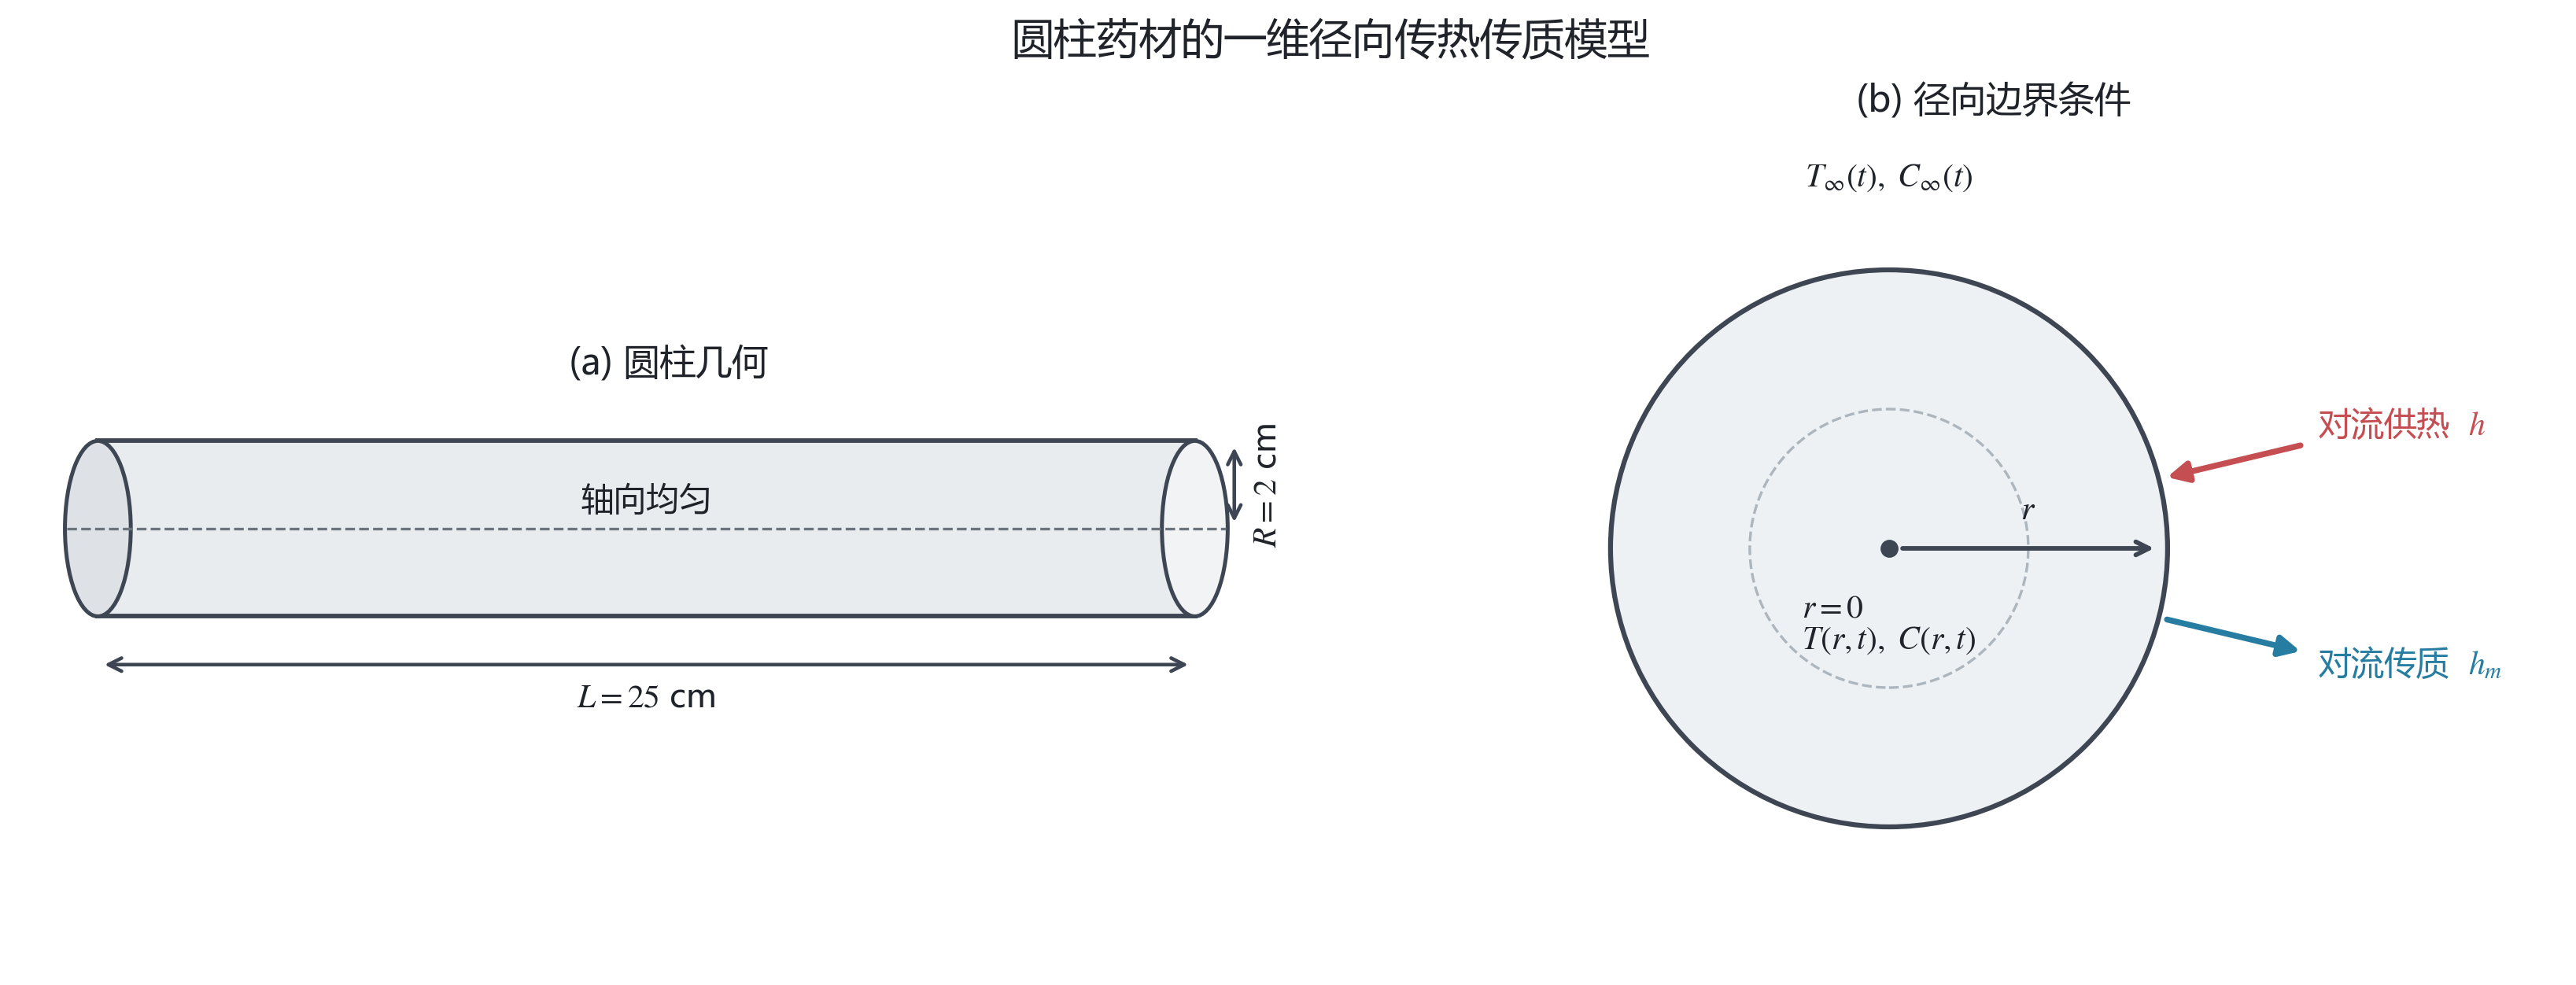
\includegraphics[width=\textwidth]{../../output/problem-1/image/fig1_model_schematic.png}
  \caption{圆柱药材的一维径向传热传质模型示意}
  \label{fig:model_schematic}
\end{figure}

\subsubsection{时变边界条件的构造}

记附件 1 的相邻观测点为 $(t_i,Y_i)$、$(t_{i+1},Y_{i+1})$，其中 $Y$ 表示 $T_\infty$ 或 $C_\infty$。在两个测点之间采用分段线性插值：
\begin{equation}
Y_\infty(t)=Y_i+
\frac{Y_{i+1}-Y_i}{t_{i+1}-t_i}(t-t_i),
\qquad t_i\leq t\leq t_{i+1}.
\label{eq:linear_interp}
\end{equation}
该方法严格通过原始测点，不改变附件的 $60\,\si{s}$ 记录，也不会产生高阶插值可能出现的超调。第一问只使用 $0$ 至 $1800\,\si{s}$ 的 31 个原始时刻。

\subsection{模型建立}

\subsubsection{参数}

温度、含水率及边界变量的符号与单位见第四部分。问题一固定采用题目附录 2 给出的几何与传输参数：
\begin{equation}
\begin{gathered}
R=0.02\,\si{m},\quad L=0.25\,\si{m},\quad
\rho=820\,\si{kg/m^3},\quad c_p=2600\,\si{J/(kg\,K)},\\
k=0.36\,\si{W/(m\,K)},\quad h=25\,\si{W/(m^2\,K)},\quad
h_m=8\times10^{-7}\,\si{m/s},\\
D(C)=7\times10^{-9}\exp\left(-\frac{0.89}{C}\right)\,\si{m^2/s}.
\end{gathered}
\label{eq:diffusivity}
\end{equation}
其中，热物性在预热平衡阶段视为常数，而有效水分扩散系数随节点处的局部干基含水率变化。

\subsubsection{温度场模型}

取半径 $r$ 至 $r+\mathrm{d}r$、长度为 $L$ 的薄环形控制体，其体积为 $\mathrm{d}V=2\pi rL\,\mathrm{d}r$。由 Fourier 定律，外向导热通量为
\begin{equation}
q_r=-k\frac{\partial T}{\partial r}.
\label{eq:fourier}
\end{equation}
令能量积累率等于内侧流入减外侧流出，得
\begin{equation}
\rho c_pT_t\,2\pi rL\,\mathrm dr
=2\pi L\{rq_r(r)-(r+\mathrm dr)q_r(r+\mathrm dr)\}.
\label{eq:heat_shell_balance}
\end{equation}
式\eqref{eq:heat_shell_balance}除以控制体体积并令 $\mathrm dr\to0$，再代入式\eqref{eq:fourier}，得到圆柱坐标下的非稳态导热方程：
\begin{equation}
\rho c_p\frac{\partial T}{\partial t}
=\frac{1}{r}\frac{\partial}{\partial r}
\left(kr\frac{\partial T}{\partial r}\right),
\qquad 0<r<R.
\label{eq:heat_pde}
\end{equation}
初始条件和中心对称条件为
\begin{equation}
T(r,0)=28,\qquad
\left.\frac{\partial T}{\partial r}\right|_{r=0}=0.
\label{eq:heat_initial_center}
\end{equation}
药材表面与烘房空气之间发生对流换热，故在 $r=R$ 处施加时变第三类边界：
\begin{equation}
-k\left.\frac{\partial T}{\partial r}\right|_{r=R}
=h\bigl[T(R,t)-T_\infty(t)\bigr].
\label{eq:heat_robin}
\end{equation}

\subsubsection{水分浓度场模型}

令 $C=m_w/m_d$ 为干基含水率，$m_w$ 和 $m_d$ 分别表示局部水分质量和绝干固体质量。把绝干固体表观密度视为常数，根据 Fick 定律，水分外向通量可写为
\begin{equation}
J_{w,r}=-\rho_dD(C)\frac{\partial C}{\partial r}.
\label{eq:fick}
\end{equation}
对同一薄环形控制体作水分质量平衡，得
\begin{equation}
\rho_d C_t\,2\pi rL\,\mathrm dr
=2\pi L\{rJ_{w,r}(r)-(r+\mathrm dr)J_{w,r}(r+\mathrm dr)\}.
\label{eq:moisture_shell_balance}
\end{equation}
式\eqref{eq:moisture_shell_balance}除以控制体体积并令 $\mathrm dr\to0$，代入式\eqref{eq:fick}后约去常数 $\rho_d$，得到
\begin{equation}
\frac{\partial C}{\partial t}
=\frac{1}{r}\frac{\partial}{\partial r}
\left[rD(C)\frac{\partial C}{\partial r}\right],
\qquad 0<r<R,
\label{eq:moisture_pde}
\end{equation}
其中扩散系数 $D(C)$ 按式（\ref{eq:diffusivity}）随局部含水率更新。
初始条件和轴线条件分别为
\begin{equation}
C(r,0)=2.55,\qquad
\left.\frac{\partial C}{\partial r}\right|_{r=0}=0.
\label{eq:moisture_initial_center}
\end{equation}
表面传质边界为
\begin{equation}
-D(C)\left.\frac{\partial C}{\partial r}\right|_{r=R}
=h_m\bigl[C(R,t)-C_\infty(t)\bigr].
\label{eq:moisture_robin}
\end{equation}
初始时刻表面水分条件与空气条件不相容，这是由题设初值和环境数据共同决定的。数值计算中应保留 $C(r,0)=2.55$，使表面失水通量从首个时间步自然形成，而不应人为修改表面初值。

\subsection{求解算法}

题目要求的交付节点为 $0,0.1,\ldots,2.0\,\si{cm}$。为减小初始表面薄边界层的离散偏差，实际计算划分 $N_{\mathrm{ref}}=1600$ 个径向区间，以 $1601$ 个节点构造控制体：
\begin{equation}
r_i=i\Delta r,\qquad \Delta r=\frac{R}{N_{\mathrm{ref}}}
=1.25\times10^{-5}\,\si{m},
\qquad i=0,1,\ldots,N_{\mathrm{ref}}.
\label{eq:grid}
\end{equation}
每隔 $80$ 个细网格节点抽取一个交付节点，因此无需进行额外的空间插值。采用节点中心有限体积法。对内部节点 $i$，控制体的内、外侧面积和体积为
\begin{equation}
A_{i\pm1/2}=2\pi Lr_{i\pm1/2},\qquad
V_i=\pi L\left(r_{i+1/2}^2-r_{i-1/2}^2\right).
\label{eq:control_volume}
\end{equation}
将温度和水分方程统一写为变量 $u$、蓄积系数 $s$、扩散系数 $\Gamma$ 与边界系数 $H$ 的形式。内部控制体离散为
\begin{equation}
sV_i\frac{\mathrm du_i}{\mathrm dt}
=A_{i+1/2}\Gamma_{i+1/2}\frac{u_{i+1}-u_i}{\Delta r}
-A_{i-1/2}\Gamma_{i-1/2}\frac{u_i-u_{i-1}}{\Delta r}.
\label{eq:fv_internal}
\end{equation}
中心控制体仅保留外侧通量；表面控制体则增加对流项
\begin{equation}
sV_{N_{\mathrm{ref}}}\frac{\mathrm du_{N_{\mathrm{ref}}}}{\mathrm dt}
=A_{N_{\mathrm{ref}}-1/2}\Gamma_{N_{\mathrm{ref}}-1/2}
\frac{u_{N_{\mathrm{ref}}-1}-u_{N_{\mathrm{ref}}}}{\Delta r}
+A_RH\bigl[u_\infty(t)-u_{N_{\mathrm{ref}}}\bigr].
\label{eq:fv_surface}
\end{equation}
温度模块中 $(u,s,\Gamma,H)=(T,\rho c_p,k,h)$；水分模块中 $(u,s,\Gamma,H)=(C,1,D,h_m)$。为保证水分通量连续，界面扩散系数采用调和平均：
\begin{equation}
D_{i+1/2}=\frac{2D(C_i)D(C_{i+1})}{D(C_i)+D(C_{i+1})}.
\label{eq:harmonic_mean}
\end{equation}
时间上采用后向 Euler 格式，将每一秒划分为 $40$ 个子步，故 $\Delta t=0.025\,\si{s}$。温度子问题在每个子步形成线性三对角系统；水分子问题采用 Picard 迭代：以当前迭代值计算界面扩散系数后组装三对角系统，直至相邻迭代的最大变化小于 $10^{-12}$，最多迭代 $60$ 次。每一整数秒抽样一次 21 个交付节点，并写入题设的两个工作表。

\subsection{求解结果}

在 $1800\,\si{s}$ 内，药材表面先升温并失水，中心温度响应滞后、含水率变化较小。图\ref{fig:time_histories}给出代表性位置的演化，温度与水分的不同响应速度与式\eqref{eq:p1_fourier_numbers}的特征时间判断一致。
\begin{figure}[!htbp]
  \centering
  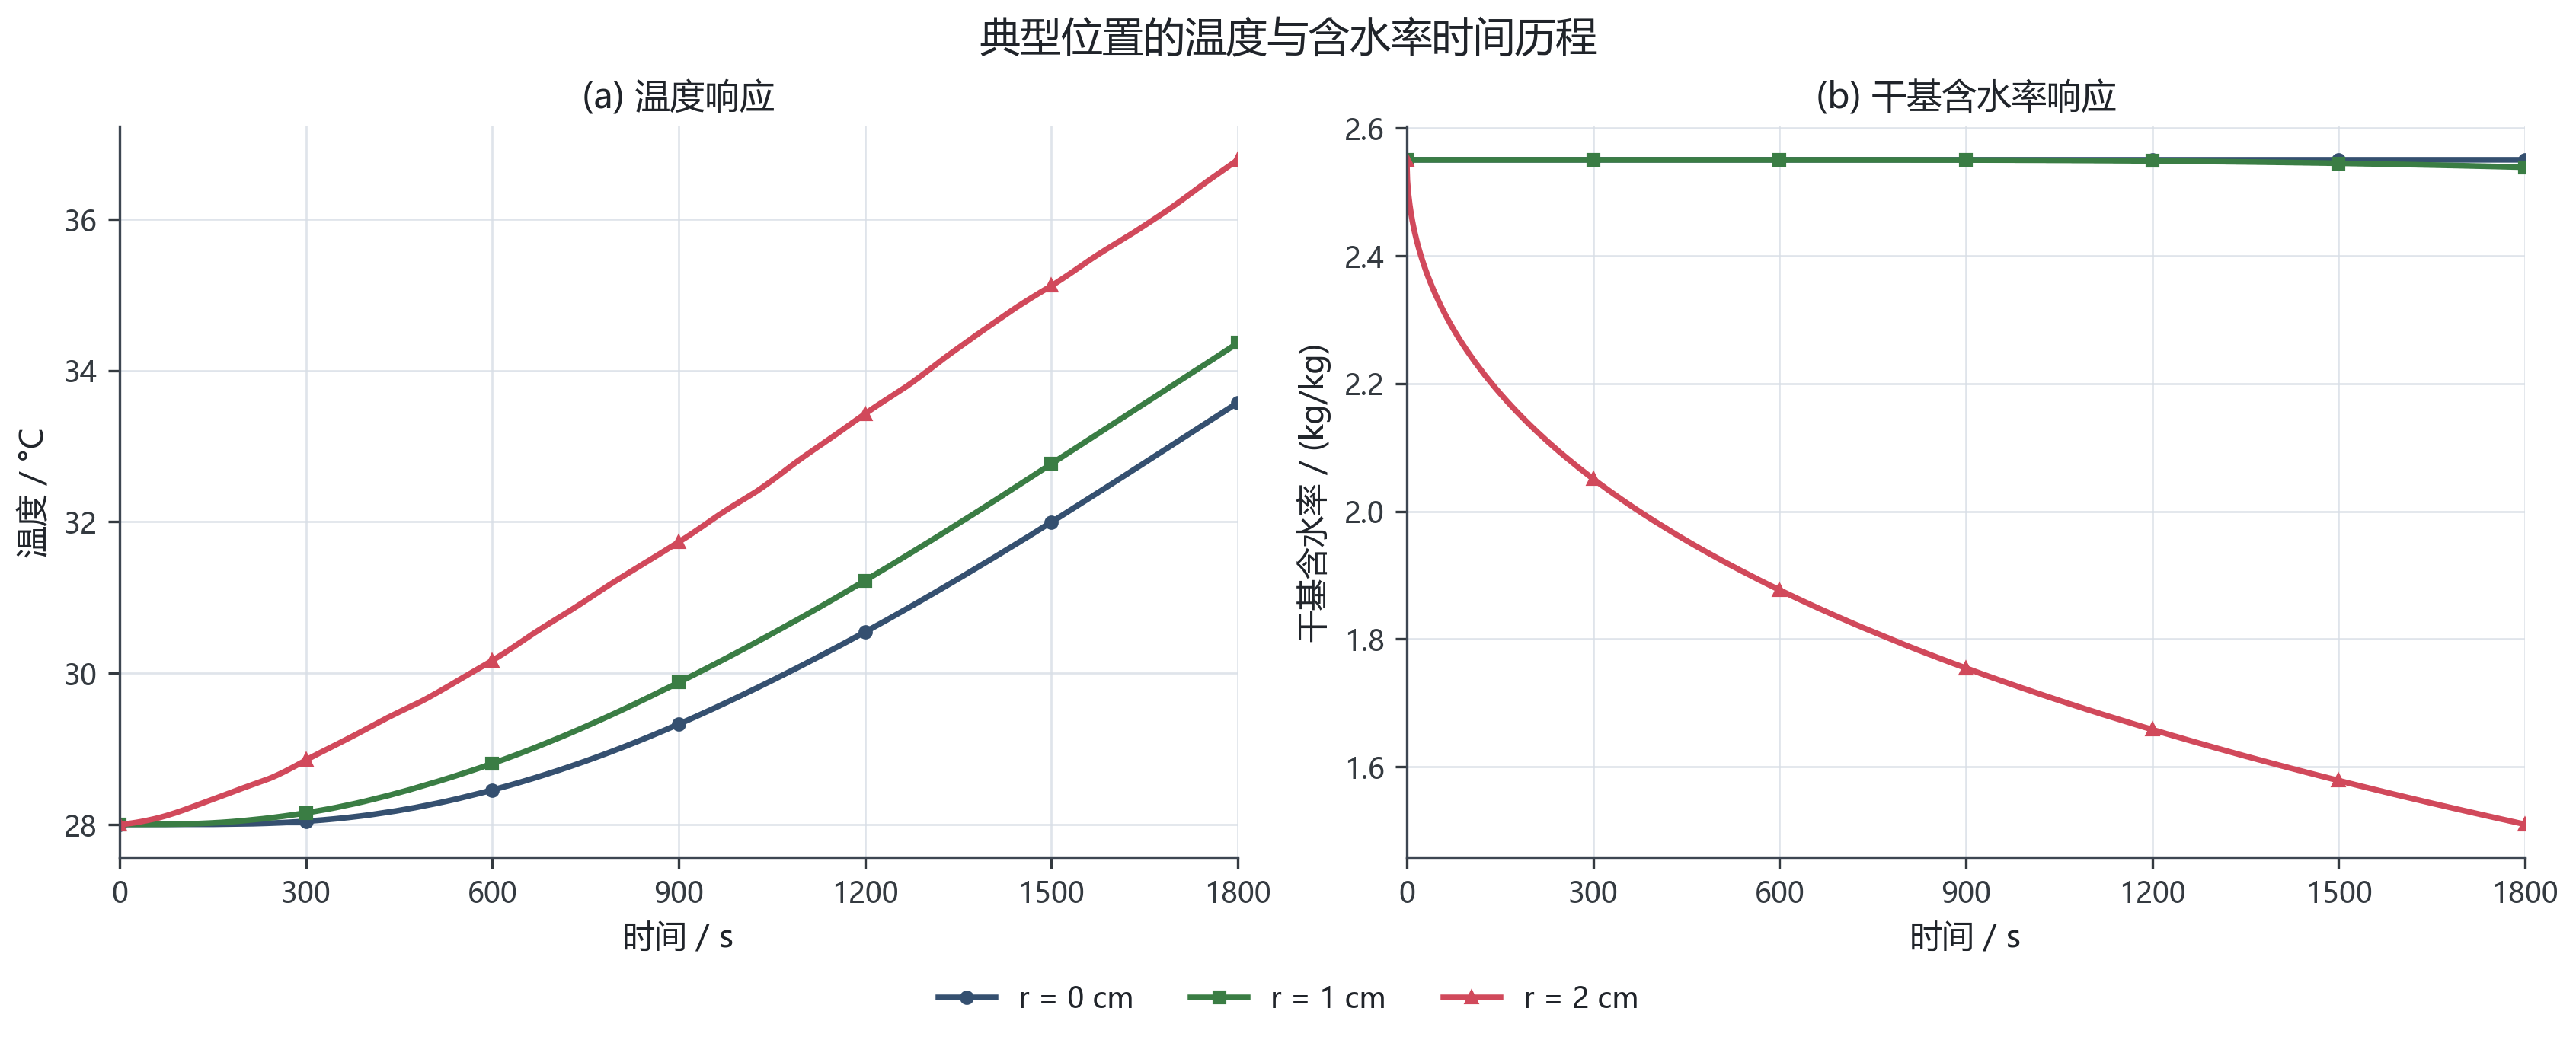
\includegraphics[width=\textwidth]{../../output/problem-1/image/fig5_time_histories.png}
  \caption{典型径向位置的温度与干基含水率时间历程}
  \label{fig:time_histories}
\end{figure}

温度场随烘房边界升温而整体上升，且表面响应快于中心。由交付节点结果可知，$1800\,\si{s}$ 时，中心温度为 $33.5754\,\si{\celsius}$，表面温度为 $36.7856\,\si{\celsius}$，两者相差 $3.2102\,\si{\celsius}$。图\ref{fig:time_histories}表明，温度沿半径方向由中心向表面递增，说明在预热平衡阶段内部温度梯度不能忽略。

水分迁移主要发生在近表面区域。$1800\,\si{s}$ 时，中心干基含水率仍为 $2.5500\,\si{kg/kg}$，而表面已降至 $1.5102\,\si{kg/kg}$；其空间分布与典型位置时间历程均显示，表面先发生明显失水，随后失水界面向内部缓慢推进。这与初始传质 Fourier 数较小的预判一致，也说明仅以平均含水率刻画该阶段无法反映表面和中心的差异。

\subsection{结果检验与解释}

数值程序从守恒性、非线性迭代收敛性、表面边界满足程度和物理趋势四个方面进行验收，结果汇总于表\ref{tab:verification}。热量与水分的守恒相对误差均低于 $10^{-4}$；每个水分时间步的 Picard 迭代均收敛，且温度、含水率的表面 Robin 残差保持在较小量级。温度和含水率的取值范围、径向单调性以及表面随时间的变化趋势亦均通过检查。

当网格由 $N=800$ 加密至 $N=1600$ 时，温度和干基含水率的最大差异分别为 $9.2\times10^{-7}\,\si{\celsius}$ 和 $1.9\times10^{-4}\,\si{kg/kg}$；后者主要发生在最初数秒的表面节点。对 $t\geq100\,\si{s}$ 的交付时刻，含水率差异小于 $6\times10^{-5}\,\si{kg/kg}$。在 $N=200$ 的时间步长检验中，将每秒子步数由 $40$ 加密至 $80$ 和由 $80$ 加密至 $160$ 时，含水率最大差异分别为 $6.5\times10^{-5}\,\si{kg/kg}$ 和 $3.3\times10^{-5}\,\si{kg/kg}$。上述加密结果支持主要时刻的数值稳定性，但不构成连续模型真解的严格误差界。输出按四位小数保留，初始 $1$--$2\,\si{s}$ 表面含水率仍有约 $10^{-4}\,\si{kg/kg}$ 的离散不确定度，不能据显示位数断言全时域四位小数均准确。

\begin{table}[H]
\centering
\caption{问题一数值验收结果}
\label{tab:verification}
\begin{tabular}{lll}
\toprule[1.2pt]
检验项目 & 结果 & 判定 \\
\midrule
热量守恒相对误差 & $9.745\times10^{-6}$ & 通过 \\
水分守恒相对误差 & $6.129\times10^{-6}$ & 通过 \\
Picard 最大迭代次数 / 残差 & $4\,/\,5.773\times10^{-15}$ & 收敛 \\
最大温度 Robin 残差 & $1.068\times10^{-4}\,\si{W/m^2}$ & 通过 \\
最大水分 Robin 残差 & $8.000\times10^{-10}\,\si{kg/(kg\,m\,s)}$ & 通过 \\
物理趋势检查 & 有限性与单调性均满足 & 通过 \\
\bottomrule[1.2pt]
\end{tabular}
\end{table}

\section{问题二的模型建立与求解}

本问沿用式\eqref{eq:linear_interp}，逐子步查询 $0$ 至 $10800\,\si{s}$ 的烘房环境，不另设恒温切换点。输入记录不作平滑或异常点删除；以题设均匀初值重新计算，新增内容是局部物性引起的两场耦合。

\subsection{模型建立}

\subsubsection{变物性与控制方程}

令 $C$ 为干基含水率，附录 3 给出的局部物性写为
\begin{equation}
\rho(C)=650+128C,\quad
c_p(C)=1450+2736\frac{C}{C+1},\quad
k(C)=0.21+0.38\frac{C}{C+1},
\label{eq:p2_thermal_properties}
\end{equation}
其中单位依次为 \si{kg/m^3}、\si{J/(kg\,K)} 和 \si{W/(m\,K)}。温度以摄氏度输出，但代入扩散系数前转换为绝对温度；有效水分扩散系数为
\begin{equation}
D(T,C)=2.4\times10^{-3}
\exp\left(-\frac{0.45}{C}\right)
\exp\left(-\frac{3850}{T+273.15}\right),\qquad C>0.
\label{eq:p2_diffusivity}
\end{equation}
定义局部体积显热容量 $a(C)=\rho(C)c_p(C)$。沿用式\eqref{eq:heat_pde}与式\eqref{eq:moisture_pde}的圆柱微元平衡，将热物性与扩散关系替换为式\eqref{eq:p2_thermal_properties}、\eqref{eq:p2_diffusivity}，得到
\begin{equation}
\begin{aligned}
a(C)\frac{\partial T}{\partial t}
&=\frac{1}{r}\frac{\partial}{\partial r}
\left[rk(C)\frac{\partial T}{\partial r}\right],\\
\frac{\partial C}{\partial t}
&=\frac{1}{r}\frac{\partial}{\partial r}
\left[rD(T,C)\frac{\partial C}{\partial r}\right],\qquad 0<r<R.
\end{aligned}
\label{eq:p2_pde}
\end{equation}
为说明变物性不能直接移出散度算子，对附录 3 的系数求导得
\begin{equation}
k_C=\frac{0.38}{(C+1)^2},\qquad
D_C=D\frac{0.45}{C^2},\qquad
D_T=D\frac{3850}{(T+273.15)^2}.
\label{eq:p2_coefficient_derivatives}
\end{equation}
将式（\ref{eq:p2_coefficient_derivatives}）代入式（\ref{eq:p2_pde}）并按乘积法则展开，可得
\begin{equation}
\begin{aligned}
a(C)T_t&=k(C)\left(T_{rr}+\frac{T_r}{r}\right)+k_CC_rT_r,\\
C_t&=D\left(C_{rr}+\frac{C_r}{r}\right)+D_C(C_r)^2+D_TT_rC_r.
\end{aligned}
\label{eq:p2_expanded_pde}
\end{equation}
式（\ref{eq:p2_expanded_pde}）中的交叉梯度项体现了温度场与含水率场的局部物性耦合；实际离散仍采用式（\ref{eq:p2_pde}）的通量形式，使界面通量守恒并避免分别逼近这些梯度乘积。
初值为 $T(r,0)=28\,\si{\celsius}$、$C(r,0)=2.55\,\si{kg/kg}$；轴线处满足零通量对称条件。表面采用时变 Robin 条件
\begin{equation}
\begin{aligned}
-k(C_s)T_r(R,t)&=h[T_s-T_\infty(t)],\\
-D(T_s,C_s)C_r(R,t)&=h_m[C_s-C_\infty(t)].
\end{aligned}
\label{eq:p2_robin}
\end{equation}
式\eqref{eq:p2_pde}不包含题目未提供参数的潜热和吸附项，故其给出的是题设经验闭合下的温湿场，而非完整热湿相变模型。

\subsubsection{有限体积离散}

采用与问题一相同的节点中心控制体，将区间数加密至 $N=3200$。式\eqref{eq:control_volume}中的面积、体积同时除以 $\pi L$，以便与问题三的长期计算统一；缩放不改变离散方程。导热与扩散系数均按式\eqref{eq:harmonic_mean}取调和平均，记
\begin{equation}
V_i=(r_i^+)^2-(r_i^-)^2,\qquad
G_{i+1/2}=\frac{2r_{i+1/2}\Gamma_{i+1/2}}{\Delta r},\qquad A_R=2R,
\label{eq:p2_scaled_geometry}
\end{equation}
其中 $r_i^-=\max(0,r_i-\Delta r/2)$、$r_i^+=\min(R,r_i+\Delta r/2)$，$\Gamma$ 取 $k$ 或 $D$。将式\eqref{eq:fv_internal}、\eqref{eq:fv_surface}按后向 Euler 离散，得
\begin{equation}
\begin{aligned}
s_iV_i\frac{u_i^{n+1}-u_i^n}{\Delta t_n}
={}&G_{i-1/2}(u_{i-1}^{n+1}-u_i^{n+1})
+G_{i+1/2}(u_{i+1}^{n+1}-u_i^{n+1})\\
&+\delta_{iN}A_RH(u_\infty^{n+1}-u_i^{n+1}).
\end{aligned}
\label{eq:p2_fvm}
\end{equation}
温度场取 $(u,s,\Gamma,H)=(T,a,k,h)$，水分场取 $(C,1,D,h_m)$。中心缺失界面的通量为零，表面保留半控制体储存量；相邻控制体共享同一界面通量。物性取新时刻迭代值，故式\eqref{eq:p2_fvm}为非线性三对角系统。

\subsection{求解算法}

每个时间步以 $T^n,C^n$ 初始化候选场；先由当前 $C$ 更新 $a,k$ 并解温度三对角方程，再由最新温度和含水率更新 $D$ 并解水分三对角方程。上述过程构成分块 Picard 不动点迭代，其停止指标为
\begin{equation}
e_{\mathrm{iter}}=\max\left\{
\frac{\|T^{(k+1)}-T^{(k)}\|_\infty}{1\,\si{\celsius}},
\frac{\|C^{(k+1)}-C^{(k)}\|_\infty}{1\,\si{kg/kg}}
\right\}.
\label{eq:p2_picard_error}
\end{equation}
当 $e_{\mathrm{iter}}<10^{-11}$ 时接受该时间步；若超过 $100$ 次仍未满足则停止并报错。生产计算的最大迭代次数为 $3$ 次，最大相邻迭代变化为 $7.6\times10^{-12}$。

初始时刻表面含水率与环境浓度并不相等，表面边界层在启动阶段较薄。为兼顾此阶段精度与三小时计算成本，按整秒编号 $m$ 采用几何斜坡步长
\begin{equation}
\Delta t_m=\min\left\{0.03125,\;0.0025\times1.3^{m-1}\right\}\,\si{s}.
\label{eq:p2_ramp_step}
\end{equation}
约第 $11\,\si{s}$ 后步长稳定为 $0.03125\,\si{s}$，总子步数约为 $3.47\times10^5$。每秒保存一次 $21$ 个交付位置的结果，并从同一数值解中抽取题设表 3、表 4，避免二次插值和重复计算。

\subsection{求解结果}

至 $3\,\si{h}$，中心与表面温差已缩小至 $0.1169\,\si{\celsius}$，但含水率差仍达 $0.7581\,\si{kg/kg}$。图\ref{fig:p2_radial_profiles}显示温度趋于均衡时，药材内部仍明显湿于表层；这说明第三问需要继续求解水分场，并以全域阈值确定终点。
\begin{figure}[!htbp]
  \centering
  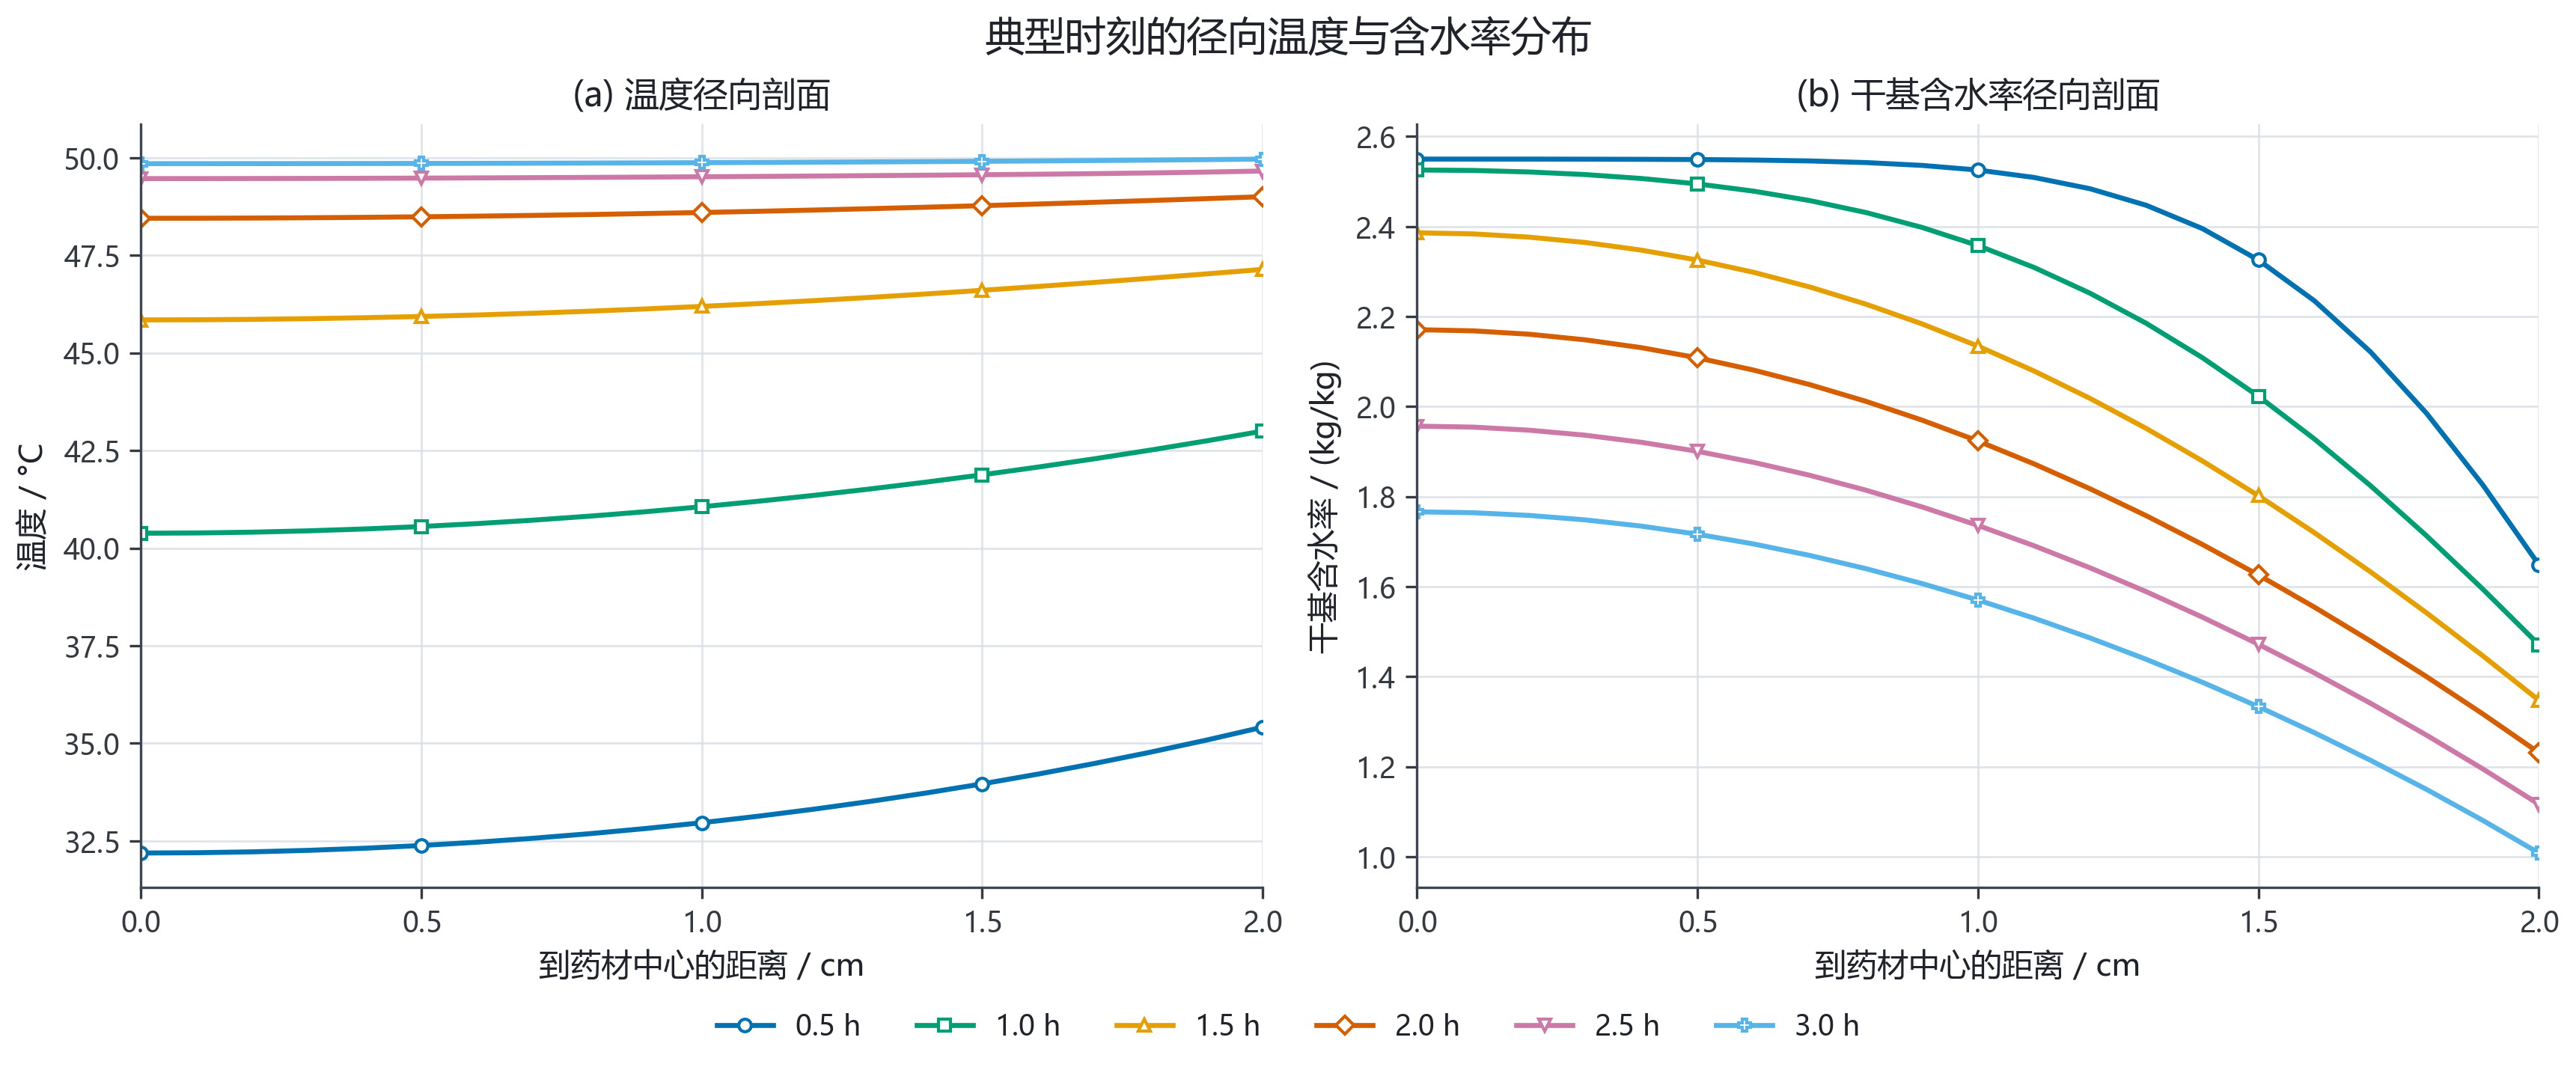
\includegraphics[width=0.96\textwidth]{../../output/problem-2/image/fig3_radial_profiles.png}
  \caption{问题二中典型时刻的径向温度与干基含水率分布}
  \label{fig:p2_radial_profiles}
\end{figure}

表\ref{tab:p2_temperature}和表\ref{tab:p2_moisture}列出题目指定位置的抽样结果。温度在 $3\,\si{h}$ 时由中心的 $49.8495\,\si{\celsius}$ 升至表面的 $49.9664\,\si{\celsius}$；相应的干基含水率由中心 $1.7662\,\si{kg/kg}$ 降至表面 $1.0081\,\si{kg/kg}$。
\begin{table}[H]
\centering
\caption{3 小时内药材温度（\si{\celsius}）}
\label{tab:p2_temperature}
{\small
\begin{tabular}{cccccc}
\toprule[1.2pt]
时间/\si{h} & $0\,\si{cm}$ & $0.5\,\si{cm}$ & $1\,\si{cm}$ & $1.5\,\si{cm}$ & $2\,\si{cm}$\\
\midrule
0.5 & 32.1893 & 32.3822 & 32.9660 & 33.9608 & 35.4130\\
1.0 & 40.3816 & 40.5536 & 41.0605 & 41.8782 & 42.9976\\
1.5 & 45.8467 & 45.9348 & 46.1929 & 46.6051 & 47.1400\\
2.0 & 48.4502 & 48.4880 & 48.5984 & 48.7735 & 49.0033\\
2.5 & 49.4670 & 49.4792 & 49.5136 & 49.5653 & 49.6609\\
3.0 & 49.8495 & 49.8553 & 49.8746 & 49.9101 & 49.9664\\
\bottomrule[1.2pt]
\end{tabular}}
\end{table}

\begin{table}[H]
\centering
\caption{3 小时内药材干基含水率（\si{kg/kg}）}
\label{tab:p2_moisture}
{\small
\begin{tabular}{cccccc}
\toprule[1.2pt]
时间/\si{h} & $0\,\si{cm}$ & $0.5\,\si{cm}$ & $1\,\si{cm}$ & $1.5\,\si{cm}$ & $2\,\si{cm}$\\
\midrule
0.5 & 2.5499 & 2.5489 & 2.5256 & 2.3257 & 1.6486\\
1.0 & 2.5257 & 2.4948 & 2.3578 & 2.0230 & 1.4711\\
1.5 & 2.3861 & 2.3256 & 2.1344 & 1.8020 & 1.3476\\
2.0 & 2.1709 & 2.1084 & 1.9236 & 1.6259 & 1.2311\\
2.5 & 1.9566 & 1.9006 & 1.7360 & 1.4720 & 1.1166\\
3.0 & 1.7662 & 1.7165 & 1.5702 & 1.3333 & 1.0081\\
\bottomrule[1.2pt]
\end{tabular}}
\end{table}

\subsection{结果检验与解释}

生产结果的空间、时间与边界检验见表\ref{tab:p2_verification}。空间网格由 $1600$ 加密至 $3200$ 时，完整交付场的最大含水率差为 $4.881\times10^{-5}\,\si{kg/kg}$；固定空间网格的时间加密比较中，最大温度差和最大含水率差分别为 $2.709\times10^{-5}\,\si{\celsius}$ 和 $9.051\times10^{-6}\,\si{kg/kg}$。两类差异均小于四位小数交付所采用的 $5\times10^{-5}$ 目标。水分与热量的离散平衡相对误差分别为 $8.706\times10^{-14}$ 和 $1.493\times10^{-12}$，表面 Robin 残差也维持在较小量级。

\begin{table}[H]
\centering
\caption{问题二数值验收结果}
\label{tab:p2_verification}
\begin{tabular}{p{0.48\textwidth}p{0.28\textwidth}c}
\toprule[1.2pt]
检验项目 & 结果 & 判定\\
\midrule
空间加密 $1600\rightarrow3200$ 的完整场最大 $|\Delta C|$ & $4.881\times10^{-5}\,\si{kg/kg}$ & 达标\\
时间加密的完整场最大 $|\Delta T|$ / $|\Delta C|$ & $2.709\times10^{-5}\,\si{\celsius}$ / $9.051\times10^{-6}\,\si{kg/kg}$ & 达标\\
水分 / 热量离散平衡相对误差 & $8.706\times10^{-14}$ / $1.493\times10^{-12}$ & 通过\\
最大温度 / 水分 Robin 残差 & $3.271\times10^{-5}\,\si{W/m^2}$ / $5.178\times10^{-11}$ & 通过\\
Picard 最大迭代次数 / 最终变化 & $3$ / $7.6\times10^{-12}$ & 收敛\\
\bottomrule[1.2pt]
\end{tabular}
\end{table}

表\ref{tab:p2_verification}中的加密差异反映相邻离散方案的自收敛性，不能等同于连续模型真解的严格误差界；守恒与边界残差检验说明离散计算一致，也不能替代真实药材的实验验证。

\section{问题三的模型建立与求解}

\subsection{长期环境与达标判据}

本问从烘干开始时的题设均匀状态独立积分，不拼接问题一或问题二的数值末状态。输入审计表明附件 1 含 $241$ 条、间隔为 $60\,\si{s}$ 的有效环境记录，覆盖 $0$ 至 $14400\,\si{s}$；记录不作平滑、裁剪或重排。主方案在观测期内采用分段线性边界，并在观测终点后以末 $30\,\si{min}$ 算术均值
\begin{equation}
\overline T_{30}=50.0133\,\si{\celsius},\qquad
\overline C_{30}=0.04999\,\si{kg/kg}
\label{eq:p3_tail_mean}
\end{equation}
为中心构造 $60\,\si{s}$ 尺度的 AR(1) 随机波动边界：
\begin{equation}
Y_\infty(14400+60m)=\overline Y_{30}+\sigma_Y z_{Y,m},\qquad
z_{Y,m+1}=\phi_Y z_{Y,m}+\varepsilon_{Y,m},\quad Y\in\{T,C\}.
\label{eq:p3_tail_boundary}
\end{equation}
其中，$\sigma_Y$ 与 $\phi_Y$ 由末段记录导出，$\varepsilon_{Y,m}$ 为相应标准化随机新息；主计算固定种子为 $0$。式（\ref{eq:p3_tail_mean}）--（\ref{eq:p3_tail_boundary}）是数据覆盖范围之外的可复现实验情景，而非附件直接观测结论。为确保终止条件覆盖整个药材，定义
\begin{equation}
g(t)=\max_{0\leq r\leq R}C(r,t)-0.15,\;\;
t_* =\inf\{t\geq0:g(t)<0\}.
\label{eq:p3_event}
\end{equation}
式\eqref{eq:p3_event}定义的是达标集合的时间下确界；连续过阈时临界点仍可能满足 $g(t_*)=0$。因此，还需在临界点之后给出经未舍入全场核验的严格达标时刻。

\subsection{模型建立}

问题三沿用问题二的附录 3 物性式\eqref{eq:p2_thermal_properties}、\eqref{eq:p2_diffusivity}，控制方程式\eqref{eq:p2_pde}及初边值条件式\eqref{eq:p2_robin}均不改变。计算从题设初值独立开始；前 $3\,\si{h}$ 与问题二对应同一连续模型，之后按式\eqref{eq:p3_tail_boundary}延长环境输入。

空间离散仍使用式\eqref{eq:p2_scaled_geometry}中的控制体和共享界面通量。为更换长期积分格式，将式\eqref{eq:p2_fvm}恢复为半离散形式：
\begin{equation}
\begin{aligned}
s_iV_i\dot u_i={}&G_{i-1/2}(u_{i-1}-u_i)+G_{i+1/2}(u_{i+1}-u_i)\\
&+\delta_{iN}A_RH(u_\infty-u_i).
\end{aligned}
\label{eq:p3_semidiscrete_fvm}
\end{equation}
变量与系数的对应关系同问题二，内部通量在全域求和时相消。新增的全域事件按式\eqref{eq:p3_event}计算：每个网格区间内采用线性重构，其最大值位于端点，因此检查全部计算节点覆盖完整重构场；这仍需通过网格加密检验对连续场的逼近。

\subsection{求解算法}

为降低长期积分的时间截断误差，采用二阶段二阶 L 稳定的 SDIRK2 隐式格式。令 $y$ 汇总温度与含水率节点值，两个阶段写为
\begin{equation}
\begin{aligned}
Y_1&=y^n+\gamma\Delta t f(t_n+\gamma\Delta t,Y_1),\\
Y_2&=y^n+(1-\gamma)\Delta t f(t_n+\gamma\Delta t,Y_1)
      +\gamma\Delta t f(t_n+\Delta t,Y_2),\\
y^{n+1}&=Y_2.
\end{aligned}
\label{eq:p3_sdirk}
\end{equation}
式（\ref{eq:p3_sdirk}）的阶段权重和为 $1$；令加权阶段时刻等于 $1/2$，二阶条件给出
\begin{equation}
(1-\gamma)\gamma+\gamma=\frac12,\qquad
\gamma^2-2\gamma+\frac12=0,\qquad
\gamma=1-\frac{1}{\sqrt2}.
\label{eq:p3_gamma_derivation}
\end{equation}
将该格式作用于试验方程 $y'=\lambda y$，消去两个阶段可得稳定函数
\begin{equation}
\mathcal R(z)=\frac{1+(1-2\gamma)z}{(1-\gamma z)^2},\qquad
z=\lambda\Delta t,\qquad
\lim_{z\to-\infty}\mathcal R(z)=0.
\label{eq:p3_stability_function}
\end{equation}
式（\ref{eq:p3_stability_function}）表明高刚性模态会被衰减，适合细径向网格下的长期扩散计算；该稳定性结论仍需由独立时间加密检验其精度。
每个阶段以分块 Picard 迭代求解：先按当前含水率更新热容和导热系数并解温度三对角方程，再按新温度与当前含水率更新扩散系数并解水分方程。迭代变化和重新代入原非线性方程的尺度化缺陷均不超过 $2\times10^{-11}$ 才接受该阶段；非正、非有限状态或迭代失败则拒绝该步并将步长减半。

主计算取 $N=12800$，网格宽 $1.5625\,\si{\micro m}$。观测期内名义步长上限为 $1\,\si{s}$，后段为 $15\,\si{s}$，并将步长截断至环境折点、$60\,\si{s}$ 输出时刻和验证截面。发现式（\ref{eq:p3_event}）的符号变化后，保存最后一个未达标的完整状态，在夹逼区间内反复重算并二分定位，直至
\begin{equation}
g(t_L)\ge0,\qquad g(t_U)<0,\qquad
t_U-t_L\le\varepsilon_t,\qquad
\widehat t_*=\frac{t_L+t_U}{2}.
\label{eq:p3_event_bracket}
\end{equation}
最后从同一未舍入状态额外积分 $0.1\,\si{s}$，再次检查全域最大值，以确认交付结束时刻满足严格小于条件。

\subsection{求解结果}

在式（\ref{eq:p3_tail_boundary}）的后续环境情景下，临界时刻估计为 $206799.708710\,\si{s}$（$57.44436353\,\si{h}$）。

取 $206799.809167\,\si{s}$ 作为严格达标交付时刻时，全域最大干基含水率为 $0.15-2.918\times10^{-8}\,\si{kg/kg}$，低于阈值。

该最大值位于圆柱中心。因此，本问给出的烘干时长为 $57.44439144\,\si{h}$，数值显示应理解为模型情景下的计算结果而非工艺安全余量。

表\ref{tab:p3_moisture}给出代表性径向含水率。末行中心值按四位小数显示为 $0.1500$，但判据始终使用未舍入值，故不与严格小于条件矛盾。
\begin{table}[H]
\centering
\caption{问题三药材烘干过程的干基含水率}
\label{tab:p3_moisture}
\begin{tabular}{cccccc}
\toprule[1.2pt]
时间/\si{h} & $0\,\si{cm}$ & $0.5\,\si{cm}$ & $1\,\si{cm}$ & $1.5\,\si{cm}$ & $2\,\si{cm}$\\
\midrule
6  & 1.0169 & 0.9881 & 0.9015 & 0.7550 & 0.5329\\
12 & 0.4560 & 0.4430 & 0.4030 & 0.3297 & 0.1642\\
18 & 0.2987 & 0.2914 & 0.2686 & 0.2252 & 0.0845\\
24 & 0.2377 & 0.2326 & 0.2166 & 0.1855 & 0.0665\\
30 & 0.2057 & 0.2018 & 0.1891 & 0.1640 & 0.0598\\
36 & 0.1858 & 0.1825 & 0.1718 & 0.1503 & 0.0566\\
42 & 0.1720 & 0.1691 & 0.1597 & 0.1407 & 0.0549\\
48 & 0.1618 & 0.1592 & 0.1507 & 0.1334 & 0.0538\\
54 & 0.1538 & 0.1514 & 0.1436 & 0.1277 & 0.0529\\
57.44439144 & 0.1500 & 0.1477 & 0.1402 & 0.1249 & 0.0527\\
\bottomrule[1.2pt]
\end{tabular}
\end{table}

图\ref{fig:p3_drying_history}显示中心、平均与表面含水率的下降历程及终点附近的情景差异。中心在全部接受时刻均为最后达标位置，但计算仍按式\eqref{eq:p3_event}检查全场；中心控制是本次解的性质，不预先代替全域判据。
\begin{figure}[!htbp]
  \centering
  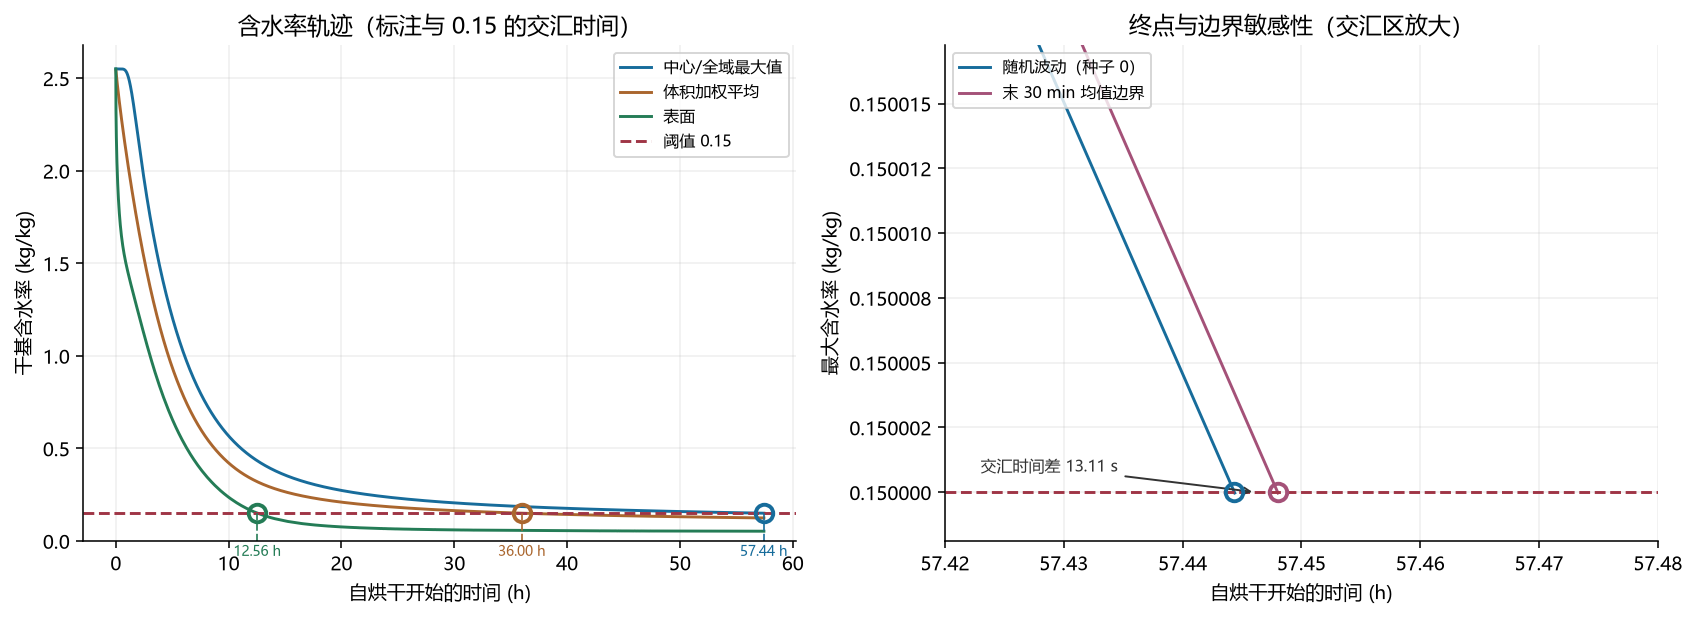
\includegraphics[width=0.95\textwidth]{../../output/problem-3/figures/drying_history.png}
  \caption{问题三的含水率干燥历程与后续边界敏感性}
  \label{fig:p3_drying_history}
\end{figure}

\subsection{结果检验与解释}

对全域事件的夹逼宽度为 $9.16\times10^{-4}\,\si{s}$；将定位容差由 $0.001\,\si{s}$ 加密至 $10^{-5}\,\si{s}$ 后，临界时刻变化为 $2.47\times10^{-4}\,\si{s}$。在所有接受时刻，最大含水率与中心值的最大差为 $4.441\times10^{-16}\,\si{kg/kg}$，径向反序的最大幅度同为舍入噪声量级，支持中心为最后达标位置的解释。

表\ref{tab:p3_verification}汇总主要数值检验。空间加密的最细两级全场含水率差为 $3.967\times10^{-5}\,\si{kg/kg}$，时间加密的最细两级差为 $1.956\times10^{-7}\,\si{kg/kg}$；两者分别检验空间和时间误差，不能混为连续模型的严格误差界。根据事件附近的下降斜率及加密结果，本计算采用约 $3\,\si{s}$ 的经验数值误差尺度，明显大于毫秒级事件定位宽度。
\begin{table}[H]
\centering
\caption{问题三主要数值验收结果}
\label{tab:p3_verification}
\begin{tabular}{p{0.51\textwidth}p{0.25\textwidth}c}
\toprule[1.2pt]
检验项目 & 结果 & 判定\\
\midrule
空间加密 $6400\rightarrow12800$ 的全场最大 $|\Delta C|$ & $3.967\times10^{-5}\,\si{kg/kg}$ & 通过\\
时间加密 $0.5\rightarrow0.25$ 的全场最大 $|\Delta C|$ & $1.956\times10^{-7}\,\si{kg/kg}$ & 通过\\
水分 / 变热容热平衡相对缺陷 & $9.275\times10^{-15}$ / $7.888\times10^{-15}$ & 通过\\
最大尺度化迭代变化 / 方程缺陷 & $2.000\times10^{-11}$ / $2.881\times10^{-12}$ & 通过\\
主方案与确定性末 $30\,\si{min}$ 均值对照的时长差 & $13.109\,\si{s}$ & 情景敏感\\
\bottomrule[1.2pt]
\end{tabular}
\end{table}

作为后续环境假设的单一敏感性对照，确定性末 $30\,\si{min}$ 均值情景的临界时刻为 $57.44800479\,\si{h}$，较主情景延长 $13.108521\,\si{s}$；该差异不能分解归因于温度或湿度中的单一因素，也不应解释为真实环境的概率置信区间。

图\ref{fig:p3_error_budget}将空间、时间离散差异及边界情景差置于同一对数尺度。后续边界的情景差大于相邻加密层级的时间差，因而本问将后续环境延拓明确作为主要情景不确定性之一，而不将其误归入求解器误差。表\ref{tab:p3_verification}的平衡缺陷只用于给定情景下的数值验收，不代替实验验证。
\begin{figure}[!htbp]
  \centering
  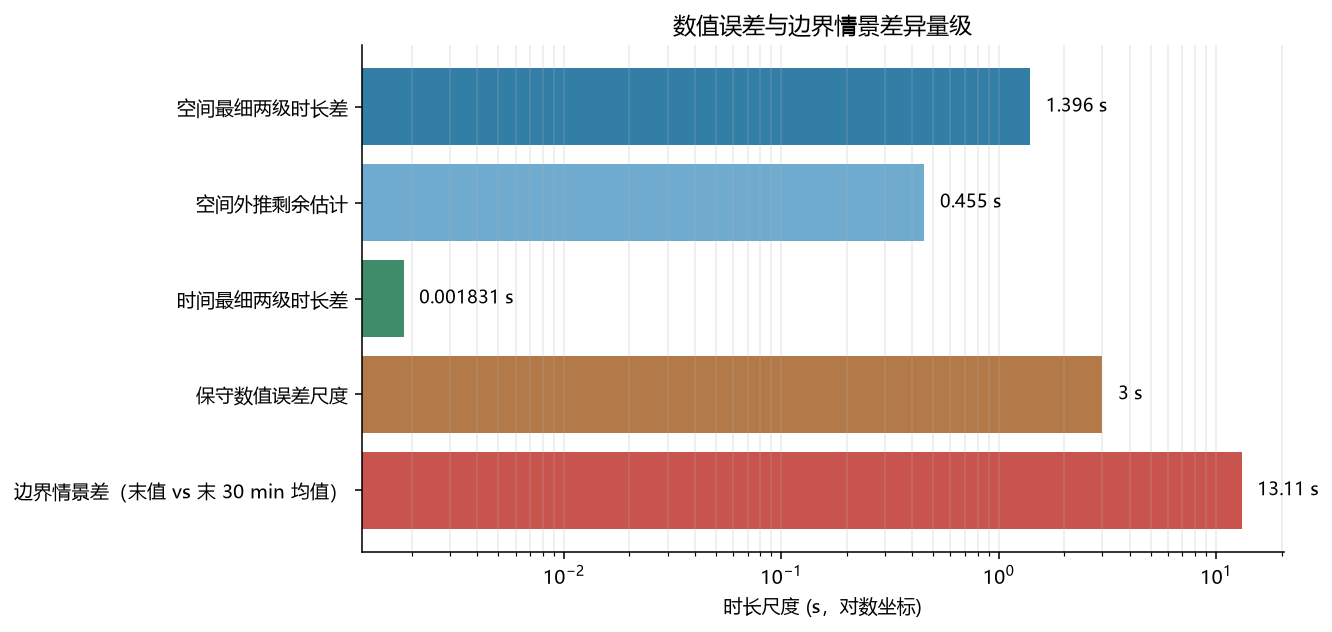
\includegraphics[width=0.82\textwidth]{../../output/problem-3/figures/error_budget.png}
  \caption{问题三数值误差尺度与后续边界情景差的比较}
  \label{fig:p3_error_budget}
\end{figure}


\section{问题四的模型建立与求解}

本问同时替换物性和几何，从题设初始均匀状态独立计算。新增推导集中于干基水分守恒、随体坐标与移动表面条件；全域事件和隐式求解沿用问题三的结构。由于固定实际位置可能在收缩后落到药材外部，交付坐标需与随体计算节点区分。

\subsection{模型建立}

\subsubsection{时变半径与环境边界}

记附件 2 相邻半径记录为 $(\tau_j,R_j)$，其中原始半径由厘米换算为米。相邻记录间采用分段线性插值：
\begin{equation}
R(t)=R_j+\frac{R_{j+1}-R_j}{\tau_{j+1}-\tau_j}(t-\tau_j),
\qquad \tau_j\le t\le\tau_{j+1}.
\label{eq:p4_radius_interp}
\end{equation}
式\eqref{eq:p4_radius_interp}严格通过全部观测点，且只在附件覆盖的 $0$ 至 $72\,\si{h}$ 内使用。附件 1 覆盖期内，$T_\infty(t)$ 与 $C_\infty(t)$ 仍按相邻记录线性插值；$4\,\si{h}$ 后主方案保持末次实测值：
\begin{equation}
T_\infty(t)=50.165\,\si{\celsius},\qquad
C_\infty(t)=0.04986\,\si{kg/kg},\qquad t>14400\,\si{s}.
\label{eq:p4_ambient_tail}
\end{equation}
图\ref{fig:p4_inputs_radius}同时展示了原始环境输入和实际半径历程。观测截止后的恒定环境是确定性情景假设，不解释为继续观测所得的事实。
\begin{figure}[!htbp]
  \centering
  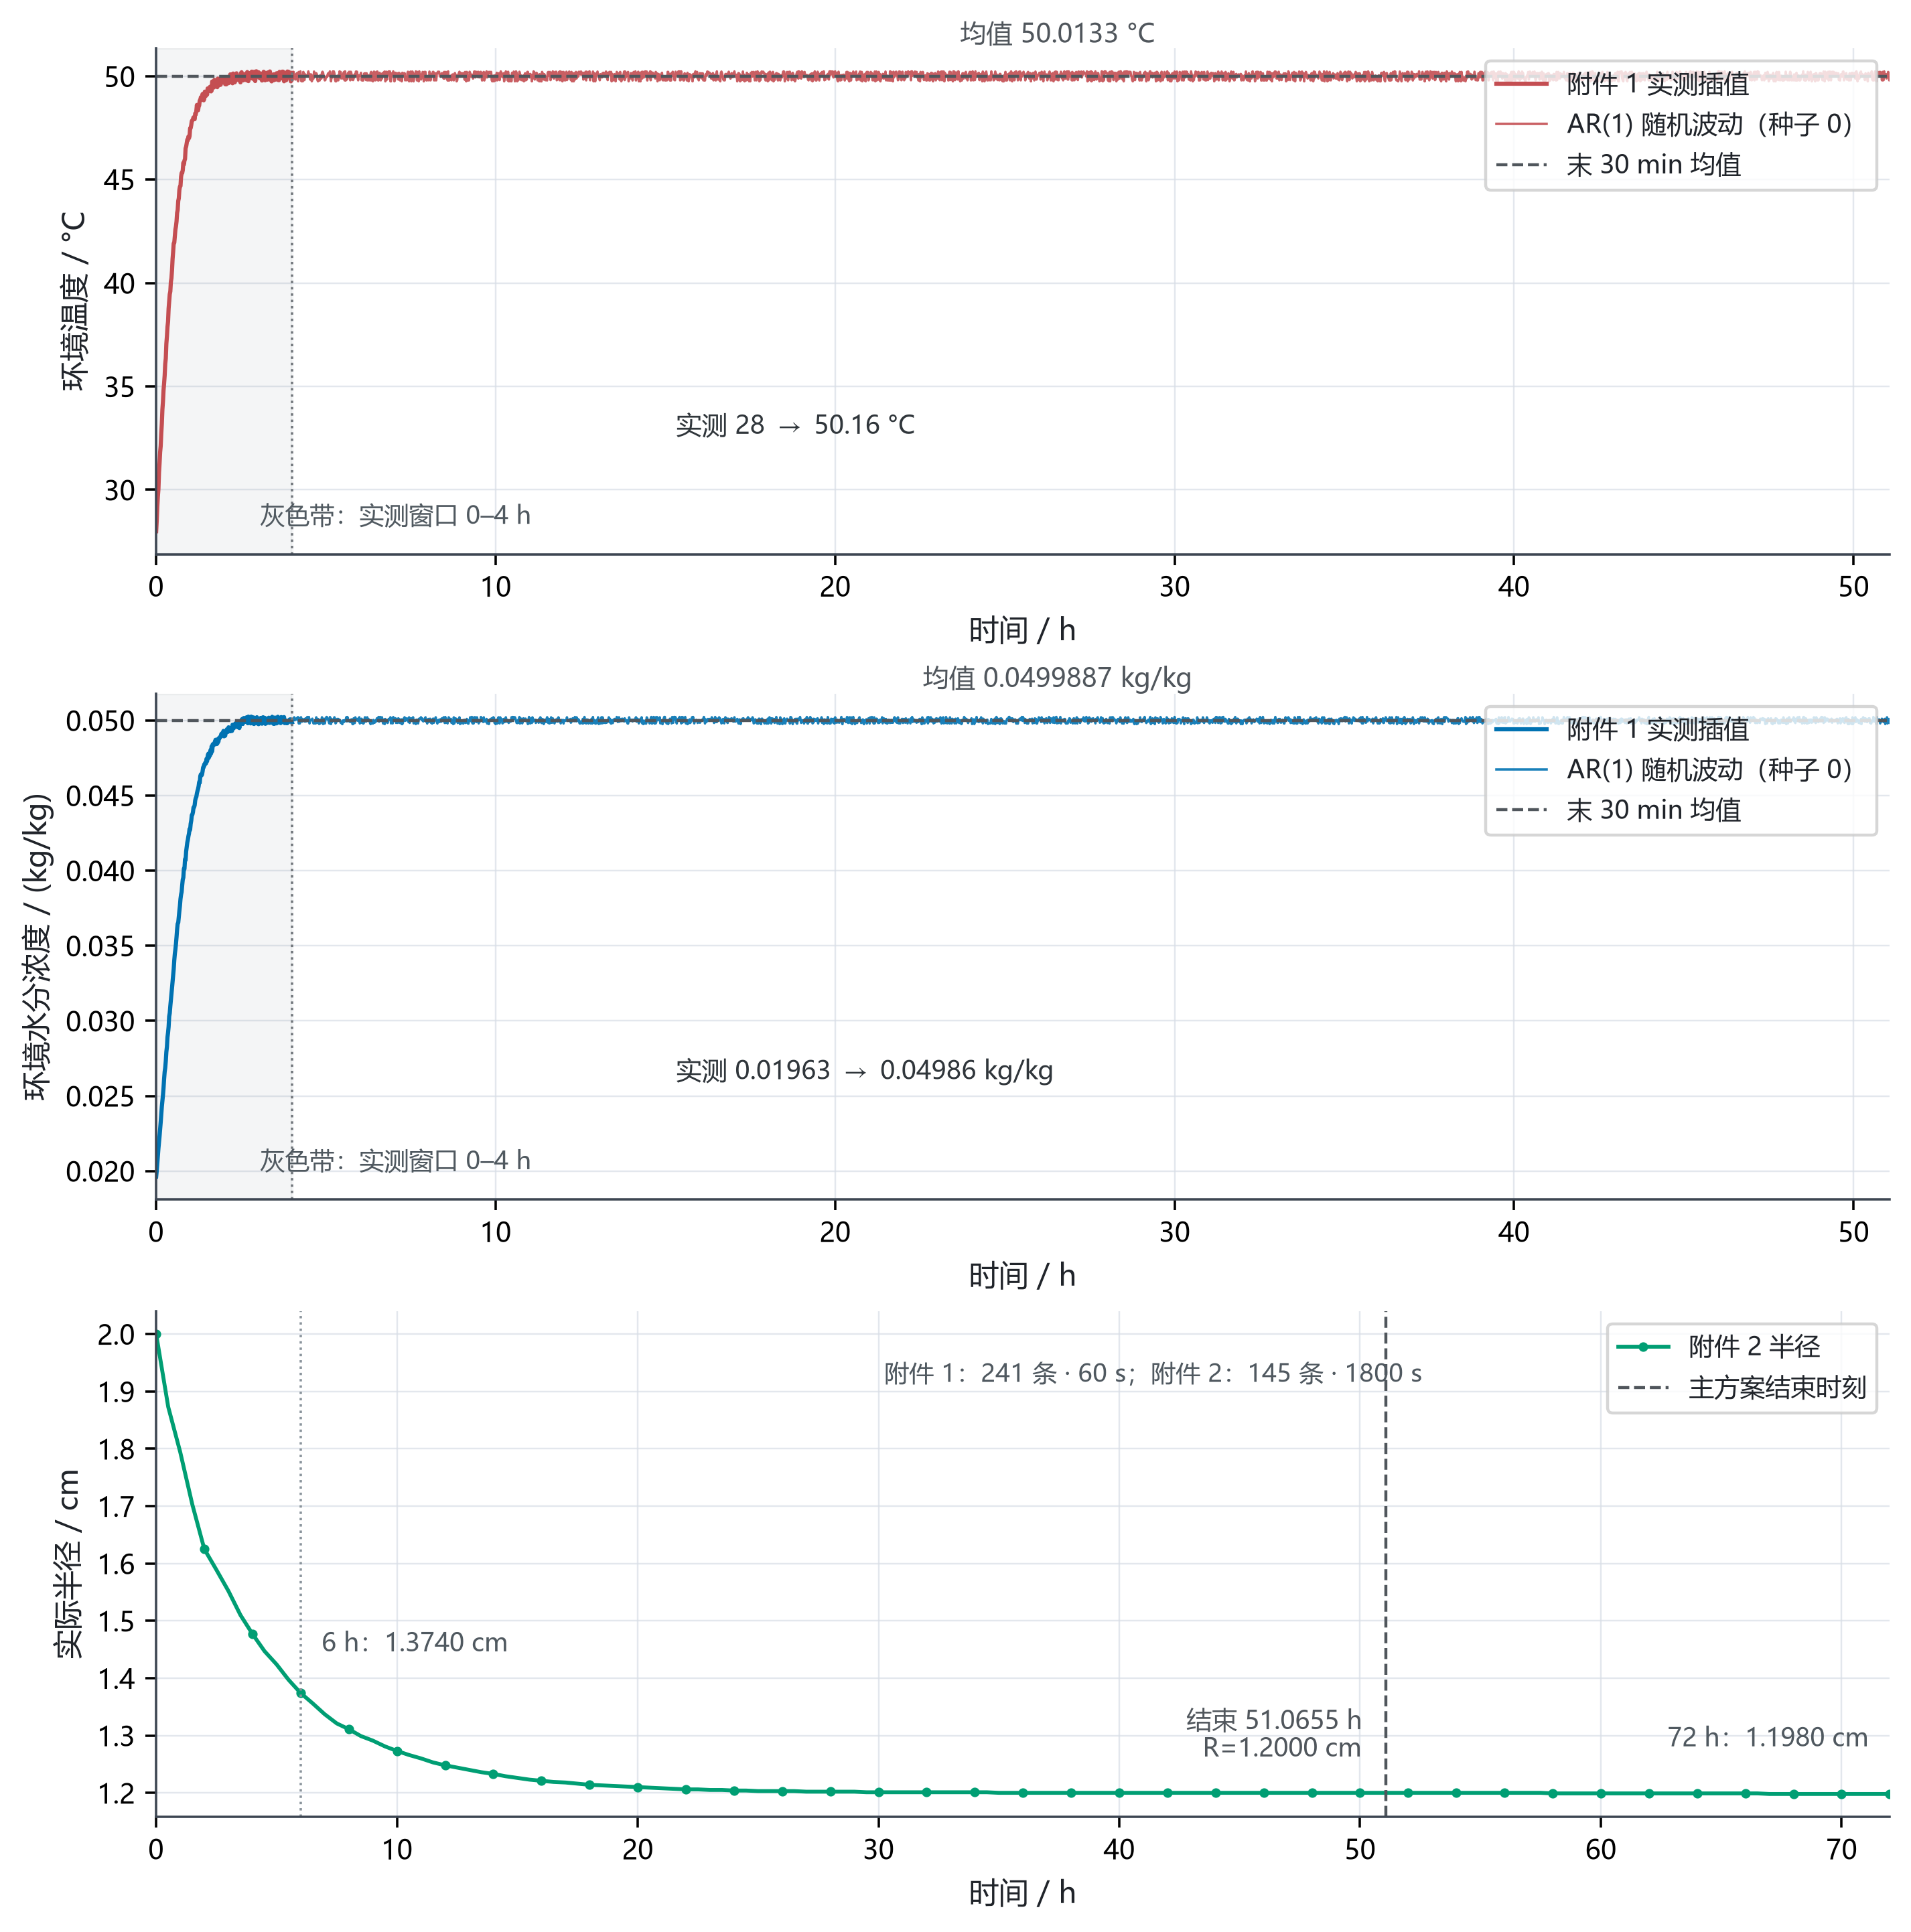
\includegraphics[width=0.92\textwidth]{../../output/problem-4/image/01_inputs_and_radius.png}
  \caption{问题四的环境输入与实测半径历程}
  \label{fig:p4_inputs_radius}
\end{figure}
\FloatBarrier

\subsubsection{附录 4 局部物性}

在局部温度和干基含水率上使用附录 4 的整套经验式：
\begin{equation}
\rho_4(X)=760+90X,\qquad
c_{p,4}(X)=1850+2150\frac{X}{1+X},\qquad
k_4(X)=0.12+0.20\frac{X}{1+X},
\label{eq:p4_thermal_properties}
\end{equation}
\begin{equation}
D_4(U,X)=4.2\times10^{-4}
\exp\!\left(-\frac{0.30}{X}\right)
\exp\!\left[-\frac{3850}{U+273.15}\right],
\qquad a_4(X)=\rho_4(X)c_{p,4}(X).
\label{eq:p4_diffusivity}
\end{equation}
其中各量采用题给 SI 单位，扩散经验式使用局部药材的绝对温度。式\eqref{eq:p4_thermal_properties}中的密度仅用于构造经验体积显热容量 $a_4$，不与后文由骨架质量守恒导出的干物质密度强行等同。

\subsubsection{收缩守恒与固定域变换}

以初始半径坐标 $a$ 标记骨架物质点，设各点按同一比例收缩：
\begin{equation}
\lambda(t)=\frac{R(t)}{R_0},\qquad
r(a,t)=\lambda(t)a,\qquad
v(r,t)=\left.\frac{\partial r}{\partial t}\right|_a
=\frac{\dot R(t)}{R(t)}r.
\label{eq:p4_material_velocity}
\end{equation}
若 $\rho_d$ 为单位当前体积内的干物质密度，则干物质连续性方程为
\begin{equation}
\frac{\partial\rho_d}{\partial t}
+\frac{1}{r}\frac{\partial}{\partial r}(r\rho_dv)=0.
\label{eq:p4_dry_mass_balance}
\end{equation}
初始干物质密度均匀且按同一比例收缩时，$\rho_d$ 仅随时间变化。将式\eqref{eq:p4_material_velocity}代入式\eqref{eq:p4_dry_mass_balance}，除以正密度并积分：
\begin{equation}
\frac{\dot\rho_d}{\rho_d}=-2\frac{\dot R}{R},
\qquad
\ln\frac{\rho_d(t)}{\rho_{d,0}}=-2\ln\frac{R(t)}{R_0}.
\label{eq:p4_dry_density_integral}
\end{equation}
对式\eqref{eq:p4_dry_density_integral}取指数，得
\begin{equation}
\rho_d(t)=\rho_{d,0}\left(\frac{R_0}{R(t)}\right)^2,
\qquad \rho_d(t)R(t)^2=\rho_{d,0}R_0^2.
\label{eq:p4_dry_density}
\end{equation}
单位当前体积内的水质量为 $\rho_dC$。令相对骨架的外向水分通量为 $J=-\rho_dD_4C_r$，水分守恒式写为
\begin{equation}
\frac{\partial(\rho_dC)}{\partial t}
+\frac{1}{r}\frac{\partial}{\partial r}(r\rho_dCv)
=-\frac{1}{r}\frac{\partial(rJ)}{\partial r}.
\label{eq:p4_water_mass_balance}
\end{equation}
按乘积法则展开式\eqref{eq:p4_water_mass_balance}，将干物质连续性项分组：
\begin{equation}
\rho_d(C_t+vC_r)
+C\left[\rho_{d,t}+\frac1r\partial_r(r\rho_dv)\right]
=-\frac1r\partial_r(rJ).
\label{eq:p4_water_cancellation}
\end{equation}
由式\eqref{eq:p4_dry_mass_balance}，式\eqref{eq:p4_water_cancellation}的方括号为零。代入 $J=-\rho_dD_4C_r$，再利用式\eqref{eq:p4_dry_density}中 $\rho_d$ 的空间均匀性，约去密度，得到物理域上的干基方程
\begin{equation}
C_t+\frac{\dot R}{R}rC_r
=\frac{1}{r}\frac{\partial}{\partial r}\left[rD_4(T,C)C_r\right].
\label{eq:p4_physical_moisture}
\end{equation}
同理，在显热近似下有
\begin{equation}
a_4(C)\left(T_t+\frac{\dot R}{R}rT_r\right)
=\frac{1}{r}\frac{\partial}{\partial r}\left[rk_4(C)T_r\right].
\label{eq:p4_physical_heat}
\end{equation}
式\eqref{eq:p4_physical_moisture}没有额外的 $C\nabla\!\cdot v$ 浓缩项，因为该项已经与干物质连续性严格抵消。

定义随体坐标和固定域场
\begin{equation}
x=\frac{r}{R(t)},\qquad
U(x,t)=T(R(t)x,t),\qquad X(x,t)=C(R(t)x,t),\qquad 0\le x\le1.
\label{eq:p4_coordinate_transform}
\end{equation}
由链式法则，任意场 $f(r,t)=F(x,t)$ 满足
\begin{equation}
f_t=F_t-x\frac{\dot R}{R}F_x,\qquad
vf_r=x\frac{\dot R}{R}F_x,\qquad
\frac{Df}{Dt}=F_t.
\label{eq:p4_material_derivative}
\end{equation}
因此物质平流与网格运动恰好抵消，同时圆柱散度项变换为
\begin{equation}
\frac{1}{r}\partial_r(r\Gamma f_r)
=\frac{1}{R(t)^2x}\partial_x(x\Gamma F_x).
\label{eq:p4_divergence_transform}
\end{equation}
最终在固定域上得到主控制方程
\begin{equation}
\boxed{\begin{aligned}
a_4(X)U_t&=\frac{1}{R(t)^2x}\frac{\partial}{\partial x}
\left[xk_4(X)U_x\right],\\
X_t&=\frac{1}{R(t)^2x}\frac{\partial}{\partial x}
\left[xD_4(U,X)X_x\right].
\end{aligned}}
\label{eq:p4_fixed_domain_pdes}
\end{equation}
式\eqref{eq:p4_fixed_domain_pdes}虽不显含 $\dot R$，但收缩仍通过 $R(t)^{-2}$ 改变内部传输尺度，并通过当前表面位置改变边界交换强度。

\subsubsection{初边值条件与达标事件}

固定域上的初始条件、轴线对称条件和实际表面 Robin 条件为
\begin{equation}
U(x,0)=28,\quad X(x,0)=2.55,\quad
U_x(0,t)=X_x(0,t)=0,
\label{eq:p4_initial_center}
\end{equation}
\begin{equation}
-\frac{k_4(X_s)}{R(t)}U_x(1,t)=h[U_s-T_\infty(t)],\qquad
-\frac{D_4(U_s,X_s)}{R(t)}X_x(1,t)=h_m[X_s-C_\infty(t)].
\label{eq:p4_robin}
\end{equation}
其中 $U_s=U(1,t)$、$X_s=X(1,t)$，$h=25\,\si{W/(m^2\,K)}$，$h_m=8\times10^{-7}\,\si{m/s}$。由于表面随骨架运动，相对表面的骨架速度为零，式\eqref{eq:p4_robin}中不应再次附加收缩携带通量。

全域达标函数及临界时刻定义为
\begin{equation}
g(t)=\max_{0\le x\le1}X(x,t)-0.15,\qquad
t_*=\inf\{t\in[0,259200]:g(t)<0\}.
\label{eq:p4_event}
\end{equation}
事件定位后取重新积分确认严格达标的上端点 $t_{\mathrm{end}}$ 作为交付结束时刻。此时全域最大值严格小于阈值。固定实际距离 $r_j$ 的输出按
\begin{equation}
x_j(t)=\frac{r_j}{R(t)},\qquad
C_j^{\mathrm{out}}(t)=X(x_j(t),t),\qquad r_j<R(t)
\label{eq:p4_output_mapping}
\end{equation}
提取；达到或超过实际半径的固定距离列留空，并另列 $X(1,t)$ 作为药材表面值。

\subsection{求解算法}

在 $[0,1]$ 上划分 $N$ 个区间，定义节点中心控制体及参考积分权重
\begin{equation}
\begin{aligned}
x_i&=i\Delta x,\qquad \Delta x=\frac1N,\\
x_i^-&=\max(0,x_i-\Delta x/2),\qquad
x_i^+=\min(1,x_i+\Delta x/2),\\
\omega_i&=(x_i^+)^2-(x_i^-)^2.
\end{aligned}
\label{eq:p4_grid}
\end{equation}
实际缩放体积为 $R(t)^2\omega_i$，且 $\sum_i\omega_i=1$。对 $\Gamma\in\{k_4,D_4\}$，界面系数采用调和平均：
\begin{equation}
\Gamma_{i+1/2}=\frac{2\Gamma_i\Gamma_{i+1}}{\Gamma_i+\Gamma_{i+1}},\qquad
G_{i+1/2}=\frac{2x_{i+1/2}\Gamma_{i+1/2}}{\Delta x}.
\label{eq:p4_conductance}
\end{equation}
以 $(f,s,\Gamma,H,f_\infty)$ 统一表示温度场 $(U,a_4,k_4,h,T_\infty)$ 和水分场 $(X,1,D_4,h_m,C_\infty)$，半离散方程为
\begin{equation}
s_iR^2\omega_i\dot f_i
=G_{i-1/2}(f_{i-1}-f_i)+G_{i+1/2}(f_{i+1}-f_i)
+\delta_{iN}2RH(f_\infty-f_i).
\label{eq:p4_semidiscrete}
\end{equation}
同一内部界面通量以相反符号装入相邻控制体，故全域求和时严格相消；中心控制体内侧面积为零，表面半控制体保留时变储存量和真实 Robin 通量。

时间积分采用式\eqref{eq:p3_sdirk}的 SDIRK2，将其中 $f$ 替换为式\eqref{eq:p4_semidiscrete}对应的移动域算子，并针对该算子重新作空间与时间加密。
每个阶段按其真实时刻查询 $R(t)$、环境边界和局部物性，并以分块 Picard 迭代交替求解温度、水分三对角系统；尺度化迭代变化与重新代入原非线性方程的缺陷均不超过 $10^{-11}$ 才接受阶段。计算步长精确截断至环境记录点、半径记录点、$60\,\si{s}$ 输出时刻和事件区间端点。

主计算采用 $N=51200$、时间倍率 $0.5$；实际步长介于 $5\times10^{-5}$ 与 $30\,\si{s}$，共接受 $14690$ 步且无拒绝步。首次发现式\eqref{eq:p4_event}变号后，从同一未达标状态局部重积分并二分，直到夹逼宽度不超过 $10^{-3}\,\si{s}$；另以 $10^{-5}\,\si{s}$ 容差作事件细化核验。

\subsection{求解结果}

主方案的临界烘干时长为 $50.82420184\,\si{h}$，严格达标结束时刻为
\begin{equation}
t_{\mathrm{end}}=182967.127075\,\si{s}=50.82420197\,\si{h}.
\label{eq:p4_end_time}
\end{equation}
该时刻的全域判据为
\begin{equation}
C_{\max}=0.149999999771844\,\si{kg/kg},\qquad
0.15-C_{\max}=2.2816\times10^{-10}\,\si{kg/kg}.
\label{eq:p4_strict_margin}
\end{equation}
最大值位于圆柱中心。表\ref{tab:p4_moisture}给出每 $6\,\si{h}$ 的代表性结果；固定距离位于当时药材外部时不列数值，表面列对应实际变化的半径。
\begin{table}[H]
\centering
\caption{问题四药材烘干过程的干基含水率}
\label{tab:p4_moisture}
{\small
\begin{tabular}{ccccc}
\toprule[1.2pt]
时间/\si{h} & $0\,\si{cm}$ & $0.5\,\si{cm}$ & $1\,\si{cm}$ & 药材表面 \\
\midrule
6  & 1.7172 & 1.5357 & 1.0217 & 0.4217 \\
12 & 0.7343 & 0.6518 & 0.4069 & 0.1667 \\
18 & 0.4066 & 0.3668 & 0.2388 & 0.0889 \\
24 & 0.2837 & 0.2599 & 0.1783 & 0.0671 \\
30 & 0.2253 & 0.2085 & 0.1488 & 0.0593 \\
36 & 0.1921 & 0.1790 & 0.1312 & 0.0558 \\
42 & 0.1706 & 0.1598 & 0.1196 & 0.0539 \\
48 & 0.1556 & 0.1463 & 0.1113 & 0.0529 \\
50.82420197 & 0.1500 & 0.1413 & 0.1081 & 0.0525 \\
\bottomrule[1.2pt]
\end{tabular}}
\end{table}
末行中心值显示为 $0.1500$ 是四位小数舍入结果，严格判据使用未舍入全场，因此不与式\eqref{eq:p4_strict_margin}矛盾。

图\ref{fig:p4_moisture_history}展示中心、全域最大值、平均值和表面值的时间历程。中心与全域最大值在数值精度内重合，表面最先失水，内部梯度随后逐步减弱。
\begin{figure}[!htbp]
  \centering
  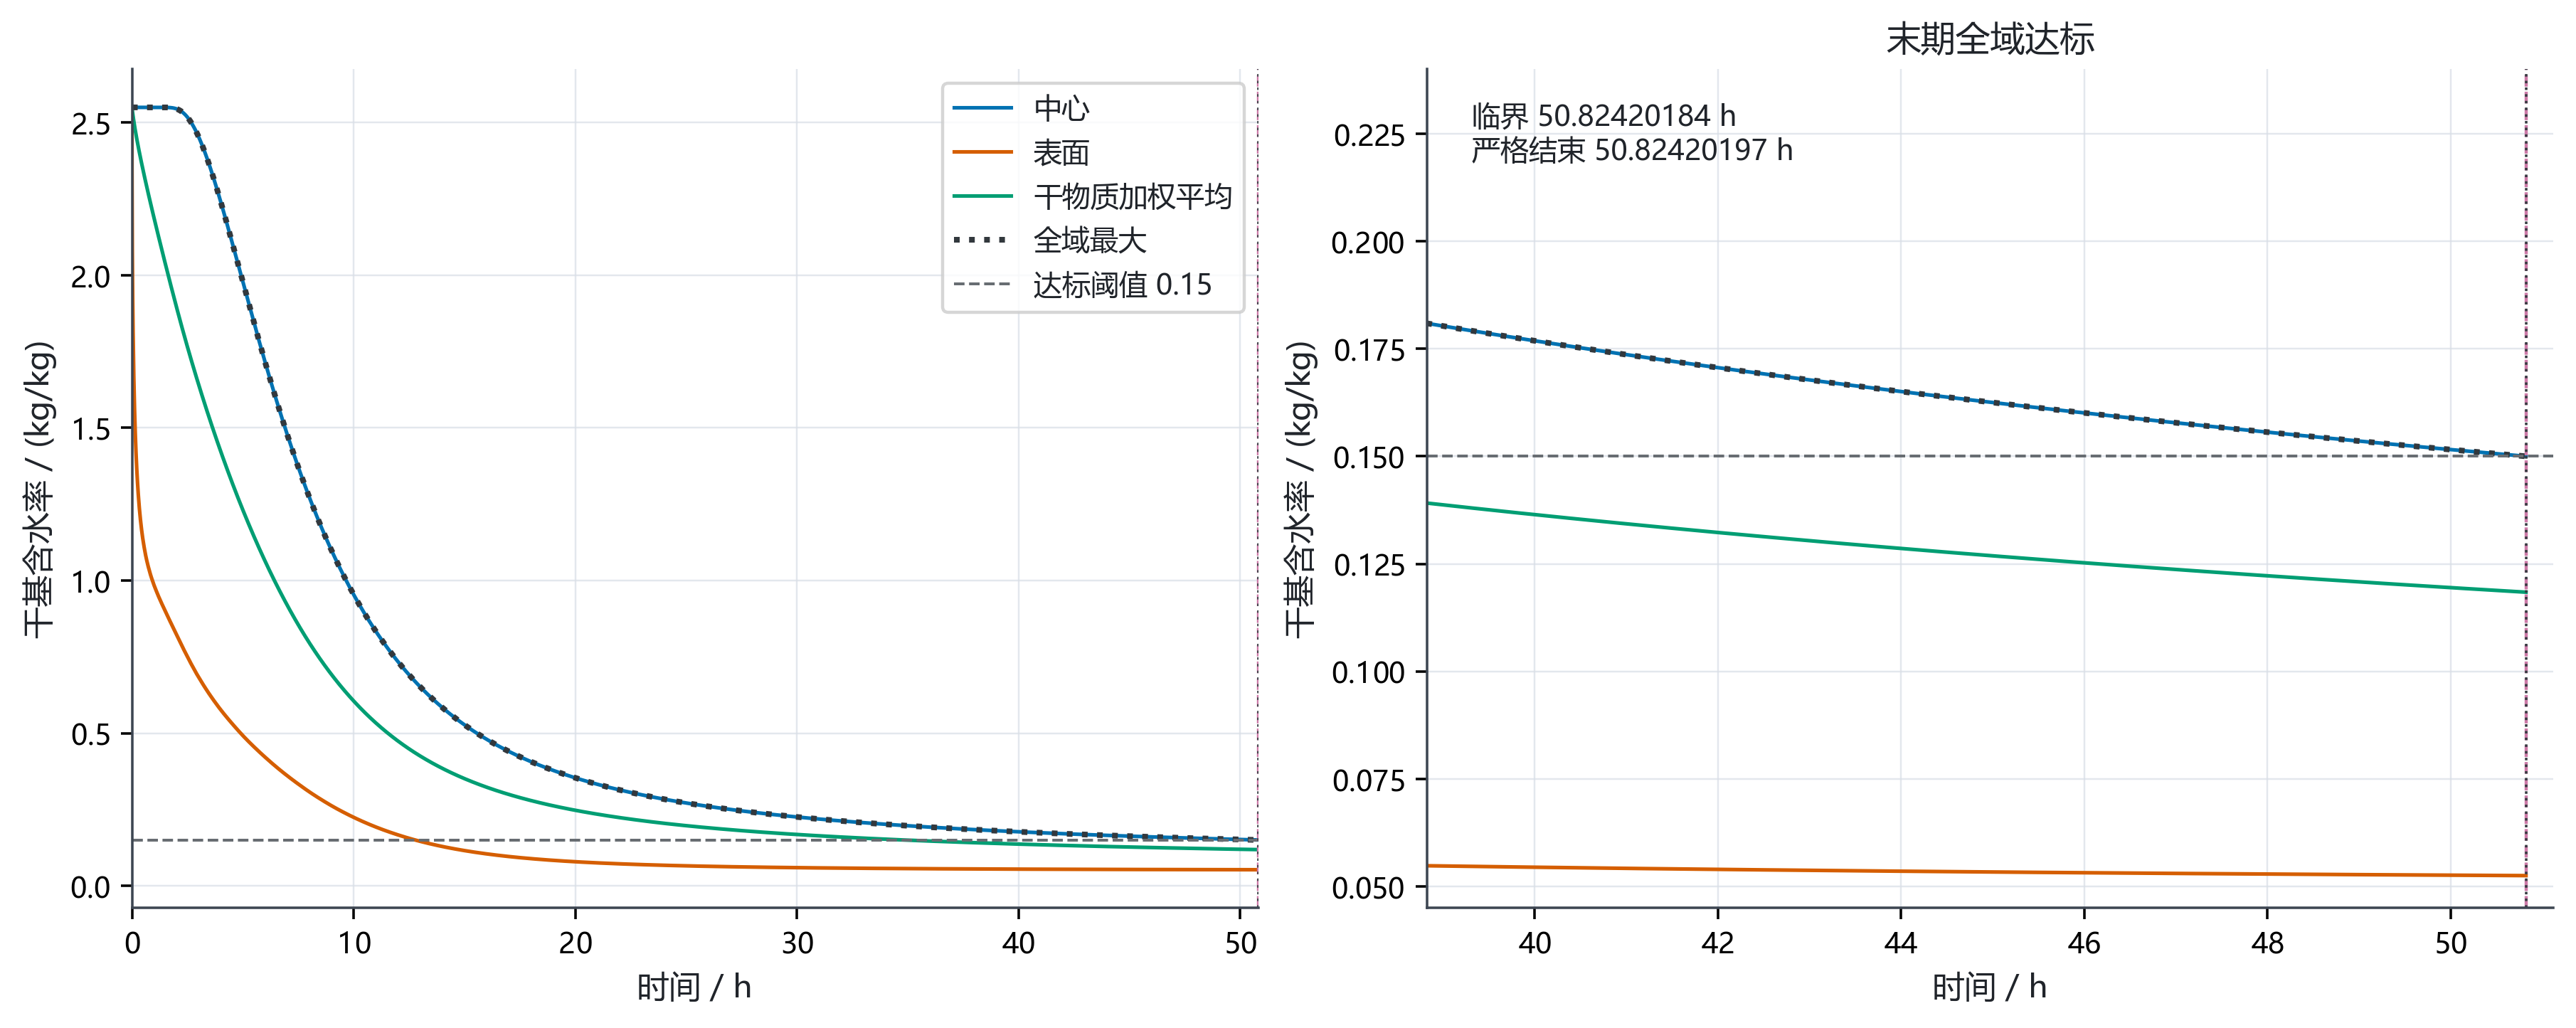
\includegraphics[width=0.88\textwidth]{../../output/problem-4/image/02_moisture_history.png}
  \caption{问题四的含水率历程与全域达标事件}
  \label{fig:p4_moisture_history}
\end{figure}


图\ref{fig:p4_space_time}将含水率展开至实际半径与时间平面，灰色区域位于药材外部。结合式\eqref{eq:p4_fixed_domain_pdes}可知，水分演化同时受局部扩散系数和时变半径控制。
\begin{figure}[!htbp]
  \centering
  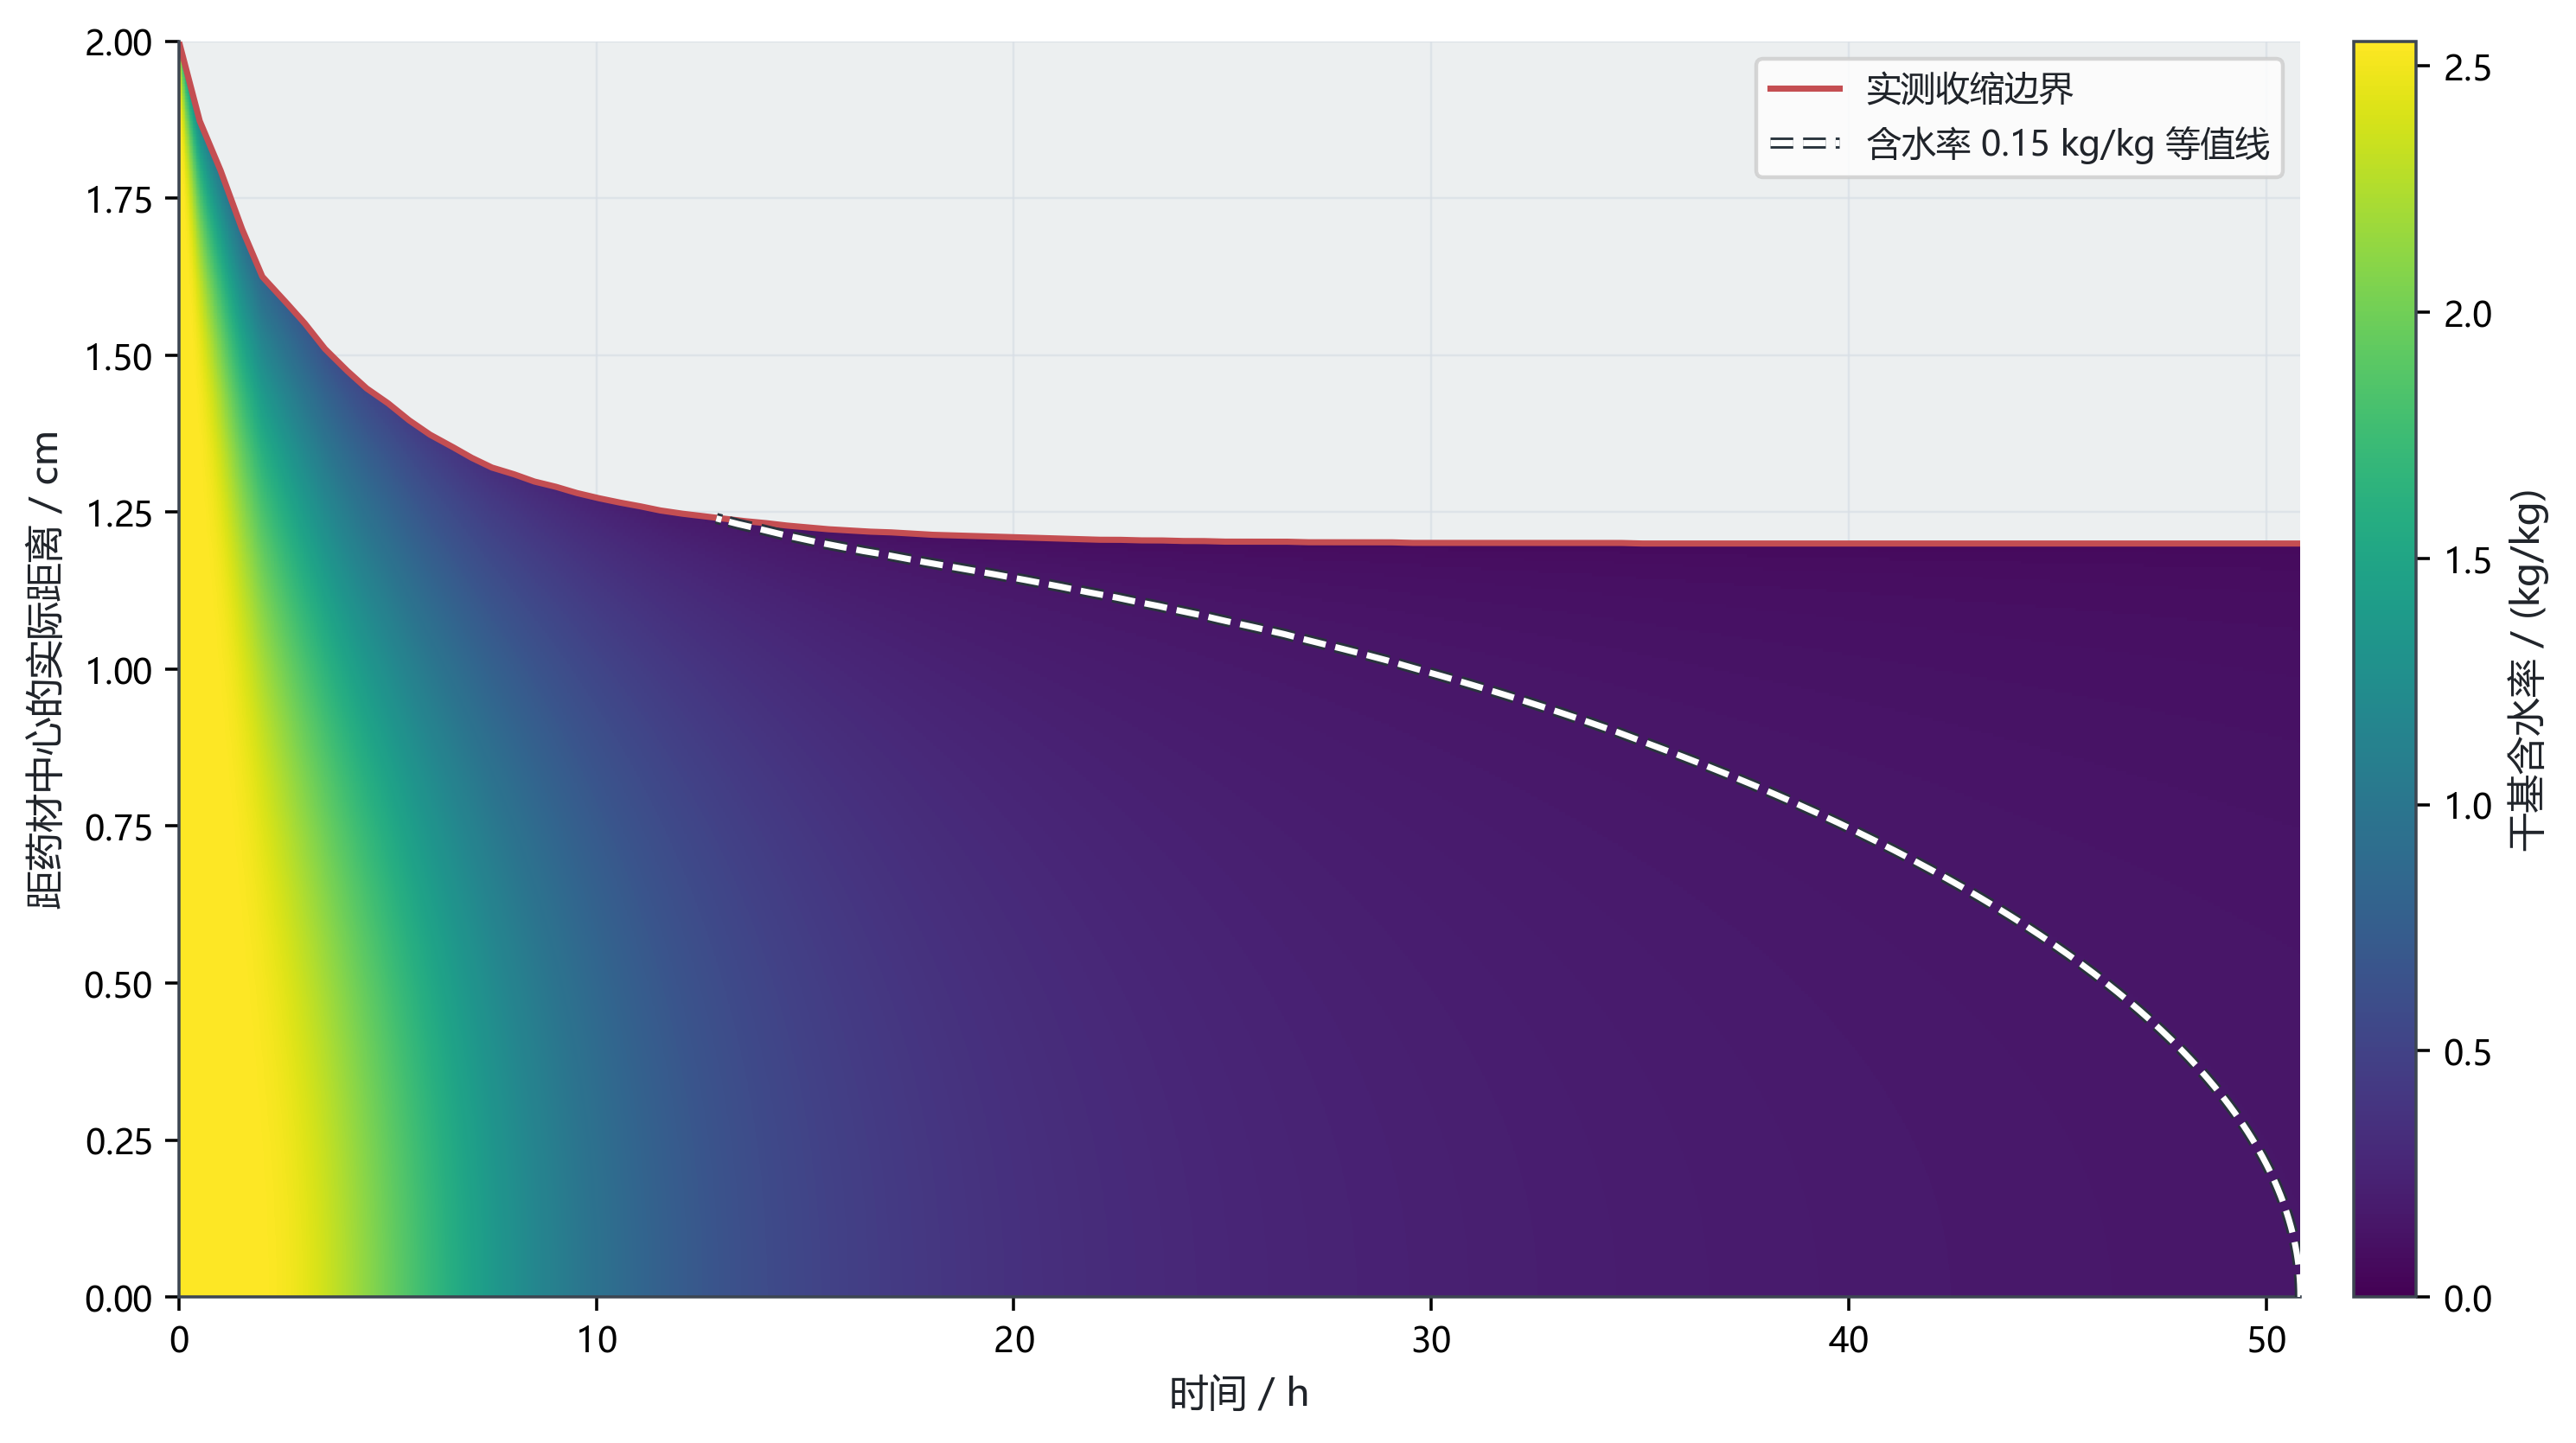
\includegraphics[width=0.90\textwidth]{../../output/problem-4/image/04_moisture_space_time.png}
  \caption{问题四移动域含水率场的时空演化}
  \label{fig:p4_space_time}
\end{figure}


\subsection{结果检验与解释}

主计算的水分、显热平衡以及非线性迭代指标为
\begin{equation}
\begin{aligned}
e_{C,\mathrm{bal}}&=1.2104\times10^{-14},&
e_{T,\mathrm{bal}}&=4.4191\times10^{-15},\\
e_{\mathrm{iter}}&=9.9959\times10^{-12},&
e_{\mathrm{eq}}&=6.3514\times10^{-14}.
\end{aligned}
\label{eq:p4_balance_metrics}
\end{equation}
事件夹逼宽度为 $9.1553\times10^{-4}\,\si{s}$，进一步收紧后临界时刻仅变化 $1.7881\times10^{-5}\,\si{s}$。

空间加密由 $N=25600$ 增至 $51200$ 时，全场含水率最大差为 $1.9265\times10^{-5}\,\si{kg/kg}$，终止时长差为 $-0.0128\,\si{s}$；时间倍率由 $0.5$ 减至 $0.25$ 时，全场含水率最大差为 $5.1523\times10^{-7}\,\si{kg/kg}$，终止时长差为 $0.0055\,\si{s}$。这些相邻离散差支持约 $1\,\si{s}$ 的经验数值误差尺度，但不是连续模型的严格误差上界。图\ref{fig:p4_convergence}汇总了空间、时间和事件定位的加密结果。
\begin{figure}[!htbp]
  \centering
  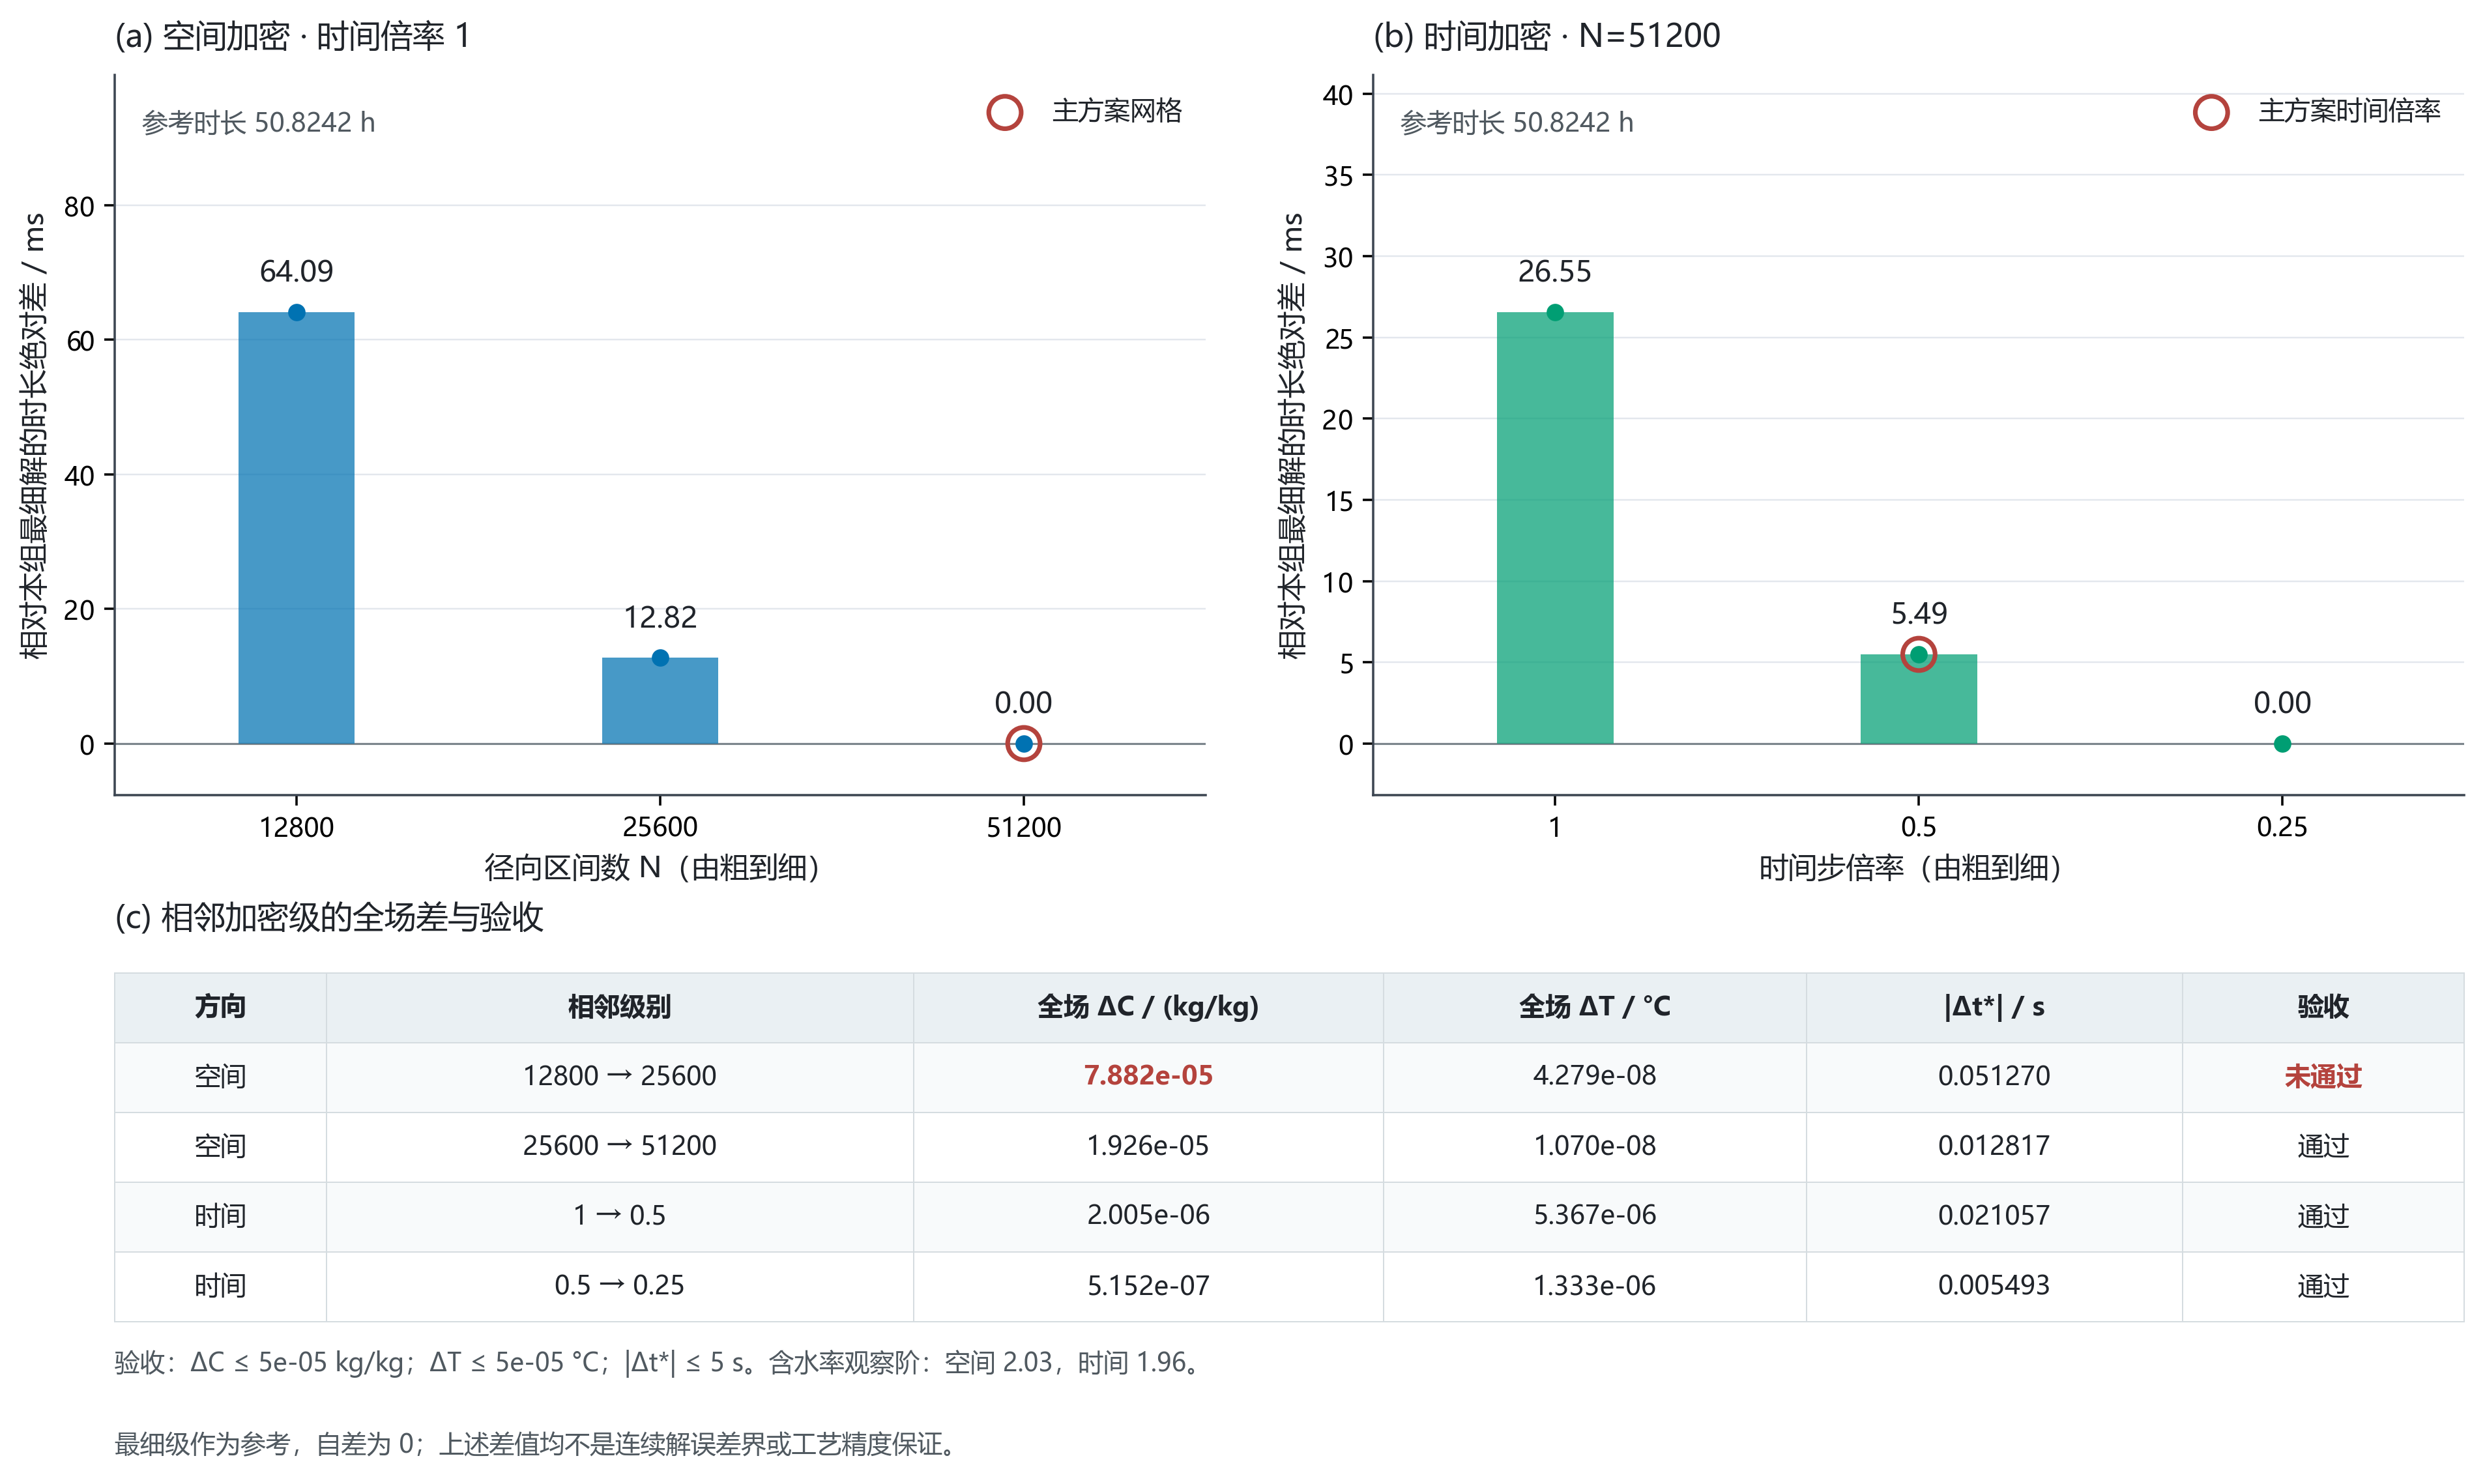
\includegraphics[width=0.88\textwidth]{../../output/problem-4/image/06_numerical_convergence.png}
  \caption{问题四的空间、时间与事件定位收敛结果}
  \label{fig:p4_convergence}
\end{figure}

为区分几何收缩、物性替换和环境延拓的影响，在相同初值下设置附录 3/4 与固定/实测半径的交叉对照。图\ref{fig:p4_scenarios}表明：附录 4 实测收缩主方案为 $50.8242\,\si{h}$；附录 3 固定半径为 $57.1694\,\si{h}$；附录 3 实测收缩为 $25.1362\,\si{h}$；附录 4 固定半径在 $72\,\si{h}$ 内仍未达标。主方案改用末 $30\,\si{min}$ 均值延拓后为 $51.0691\,\si{h}$。该交叉对照统一采用问题四的末值环境延拓；其中 $57.1694\,\si{h}$ 与问题三随机边界下的 $57.4444\,\si{h}$ 属于不同情景，不可混作同一基准。物性替换与收缩的作用存在非线性耦合，不能按末半径比例缩放或简单相加归因。
\begin{figure}[!htbp]
  \centering
  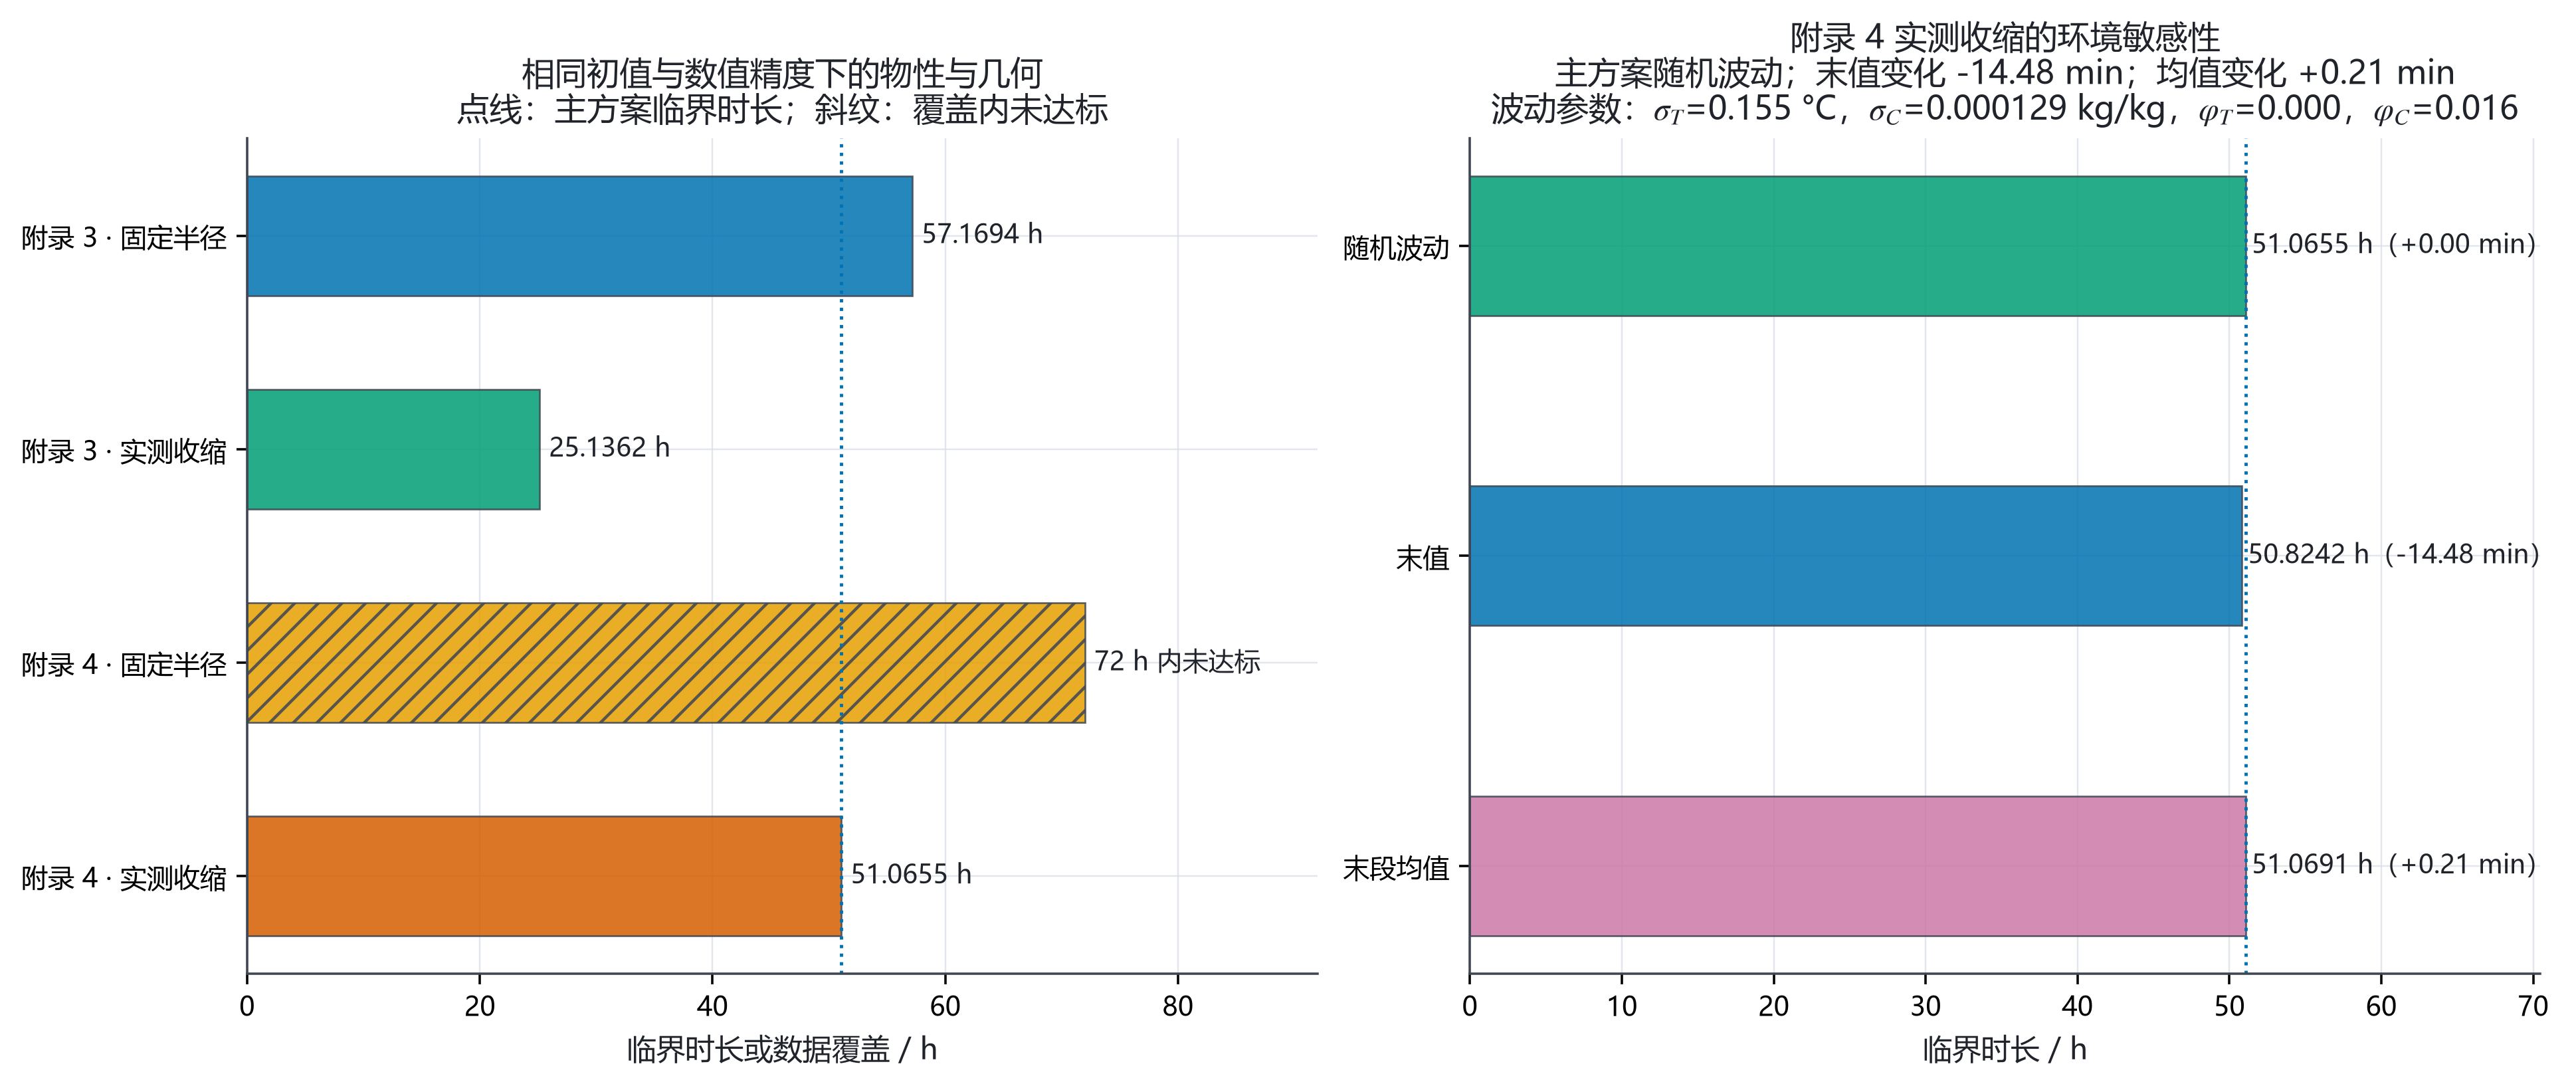
\includegraphics[width=0.90\textwidth]{../../output/problem-4/image/07_scenarios_and_sensitivity.png}
  \caption{问题四的物性、几何及后续环境情景对照}
  \label{fig:p4_scenarios}
\end{figure}

综上，数值平衡、边界重构、空间--时间加密和独立 BDF 短时对照共同支持离散求解的一致性。仍需强调：均匀内部收缩与 $4\,\si{h}$ 后环境均属于模型假设，附录 4 物性也缺少本题独立实验校准；因此 $50.8242\,\si{h}$ 应解释为既定情景下的模型计算时长，而非无需安全余量即可直接采用的工艺终点。

\clearpage
\section{模型的综合检验与误差分析}

\subsection{误差来源}
\vspace{0.08\textheight}

\subsection{敏感性分析}
\vspace{0.08\textheight}

\subsection{稳健性或统计检验}
\vspace{0.08\textheight}

\subsection{不同方法对比}
\vspace{0.08\textheight}

\clearpage
\section{模型评价、改进与推广}

\subsection{模型优点}
\vspace{0.06\textheight}

\subsection{模型局限}

问题一以固定半径圆柱、时变环境边界和水分扩散系数非线性为基础，未处理端面效应、潜热耦合及湿度至平衡含水率的换算。其余问题的局限待实际模型和结果补充后统一讨论。

\subsection{改进方向}
\vspace{0.06\textheight}

\subsection{推广与应用}
\vspace{0.06\textheight}

\section{结论}
\vspace{0.10\textheight}

\section*{参考文献}
% 待用户提供并在正文实际引用后添加；当前不列入任何条目。
\vspace{0.08\textheight}

\clearpage
\begin{appendices}
\section{文件和程序说明}
\vspace{0.10\textheight}

\section{核心代码}
\vspace{0.10\textheight}

\section{补充数据及图表}
\vspace{0.10\textheight}
\end{appendices}

\CumcmAIUsed{文稿初稿整理、公式排版辅助和程序调试}

\end{document}
